\documentclass[dvipdfmx,aspectratio=169]{beamer}
\usepackage{pxjahyper}							%しおりの文字化けを防ぐ
\renewcommand{\kanjifamilydefault}{\gtdefault}	%日本語フォントをゴシックに
\usepackage{graphics}							%各種画像の張り込み
\usepackage{amsmath,amssymb,mathtools}					%標準数式表現を拡大する
\usepackage{ulem}
\usepackage{ascmac,fancybox}
\usetheme[
	block=fill,
	progressbar=foot,
	numbering=fraction,
	subsectionpage=progressbar
]{Metropolis}
\usefonttheme{professionalfonts}

\usepackage{here}
\usepackage{booktabs}

\usepackage{tikz}
\usetikzlibrary{positioning}
\usepackage{color}

\newcommand{\highlight}[2][yellow]{\tikz[baseline=(x.base)]{\node[rectangle,rounded corners,fill=#1!10](x){#2};}}
\newcommand{\highlightcap}[3][yellow]{\tikz[baseline=(x.base)]{\node[rectangle,rounded corners,fill=#1!10](x){#2} node[below of=x, color=#1]{#3};}}

\title{ディープラーニングの仕組みを知ろう!}
\subtitle{第1回 人工知能勉強会 数学編}
\author{Shion MORISHITA}
\institute{}
\date{June 15, 2024}

\subject{\LaTeX{}+Beamer}
\begin{document}
	%タイトル
	\begin{frame}[plain]
	    \maketitle
	\end{frame}
		
	\begin{frame}[shrink]{目次}
		\vspace{1em}
		\tableofcontents
	\end{frame}
	
	\section{はじめに}
	\begin{frame}{目的}
		\begin{itemize}
			\item ニューラルネットワークの構造を数理的に理解する
			\item ニューラルネットワークや、その学習方法について理解するために必要な数学の基礎を復習・理解する
		\end{itemize}
	\end{frame}

	\section{ニューラルネットワークの考え方}
	\subsection{ニューロン}
	\begin{frame}{ニューロン$ = $神経細胞}
		\begin{itemize}
			\item 互いに結びついてネットワークを構築することで、\\さまざまな処理を行なっている
		\end{itemize}

		\begin{figure}
			\centering
			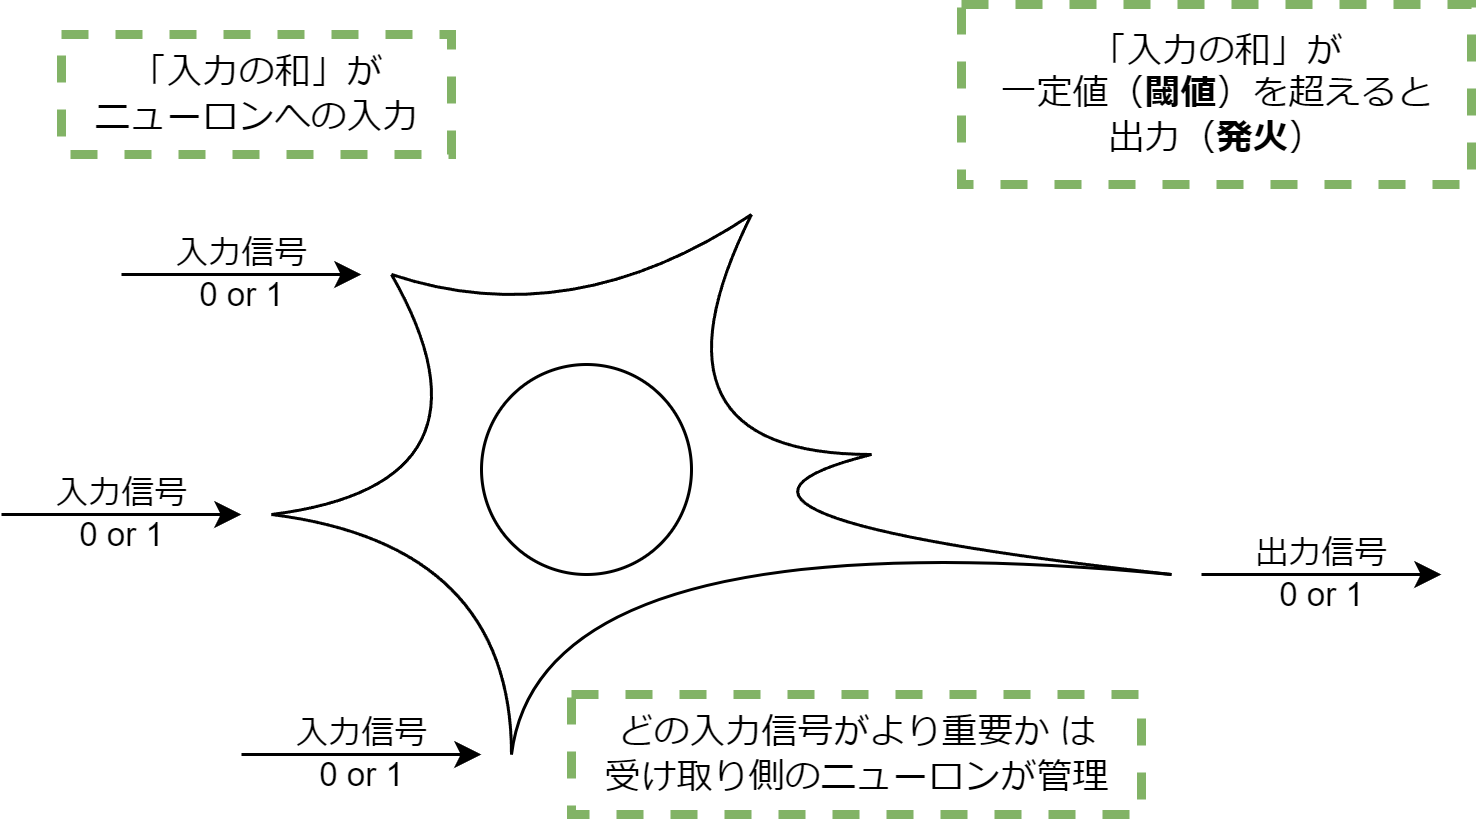
\includegraphics[width=0.6\linewidth]{img/function-of-neurons}
		\end{figure}
	\end{frame}
	
	\subsection{ニューロンの働きの数理的解釈}
	\begin{frame}{ニューロンの働きの数理的解釈}
		\begin{figure}
			\centering
			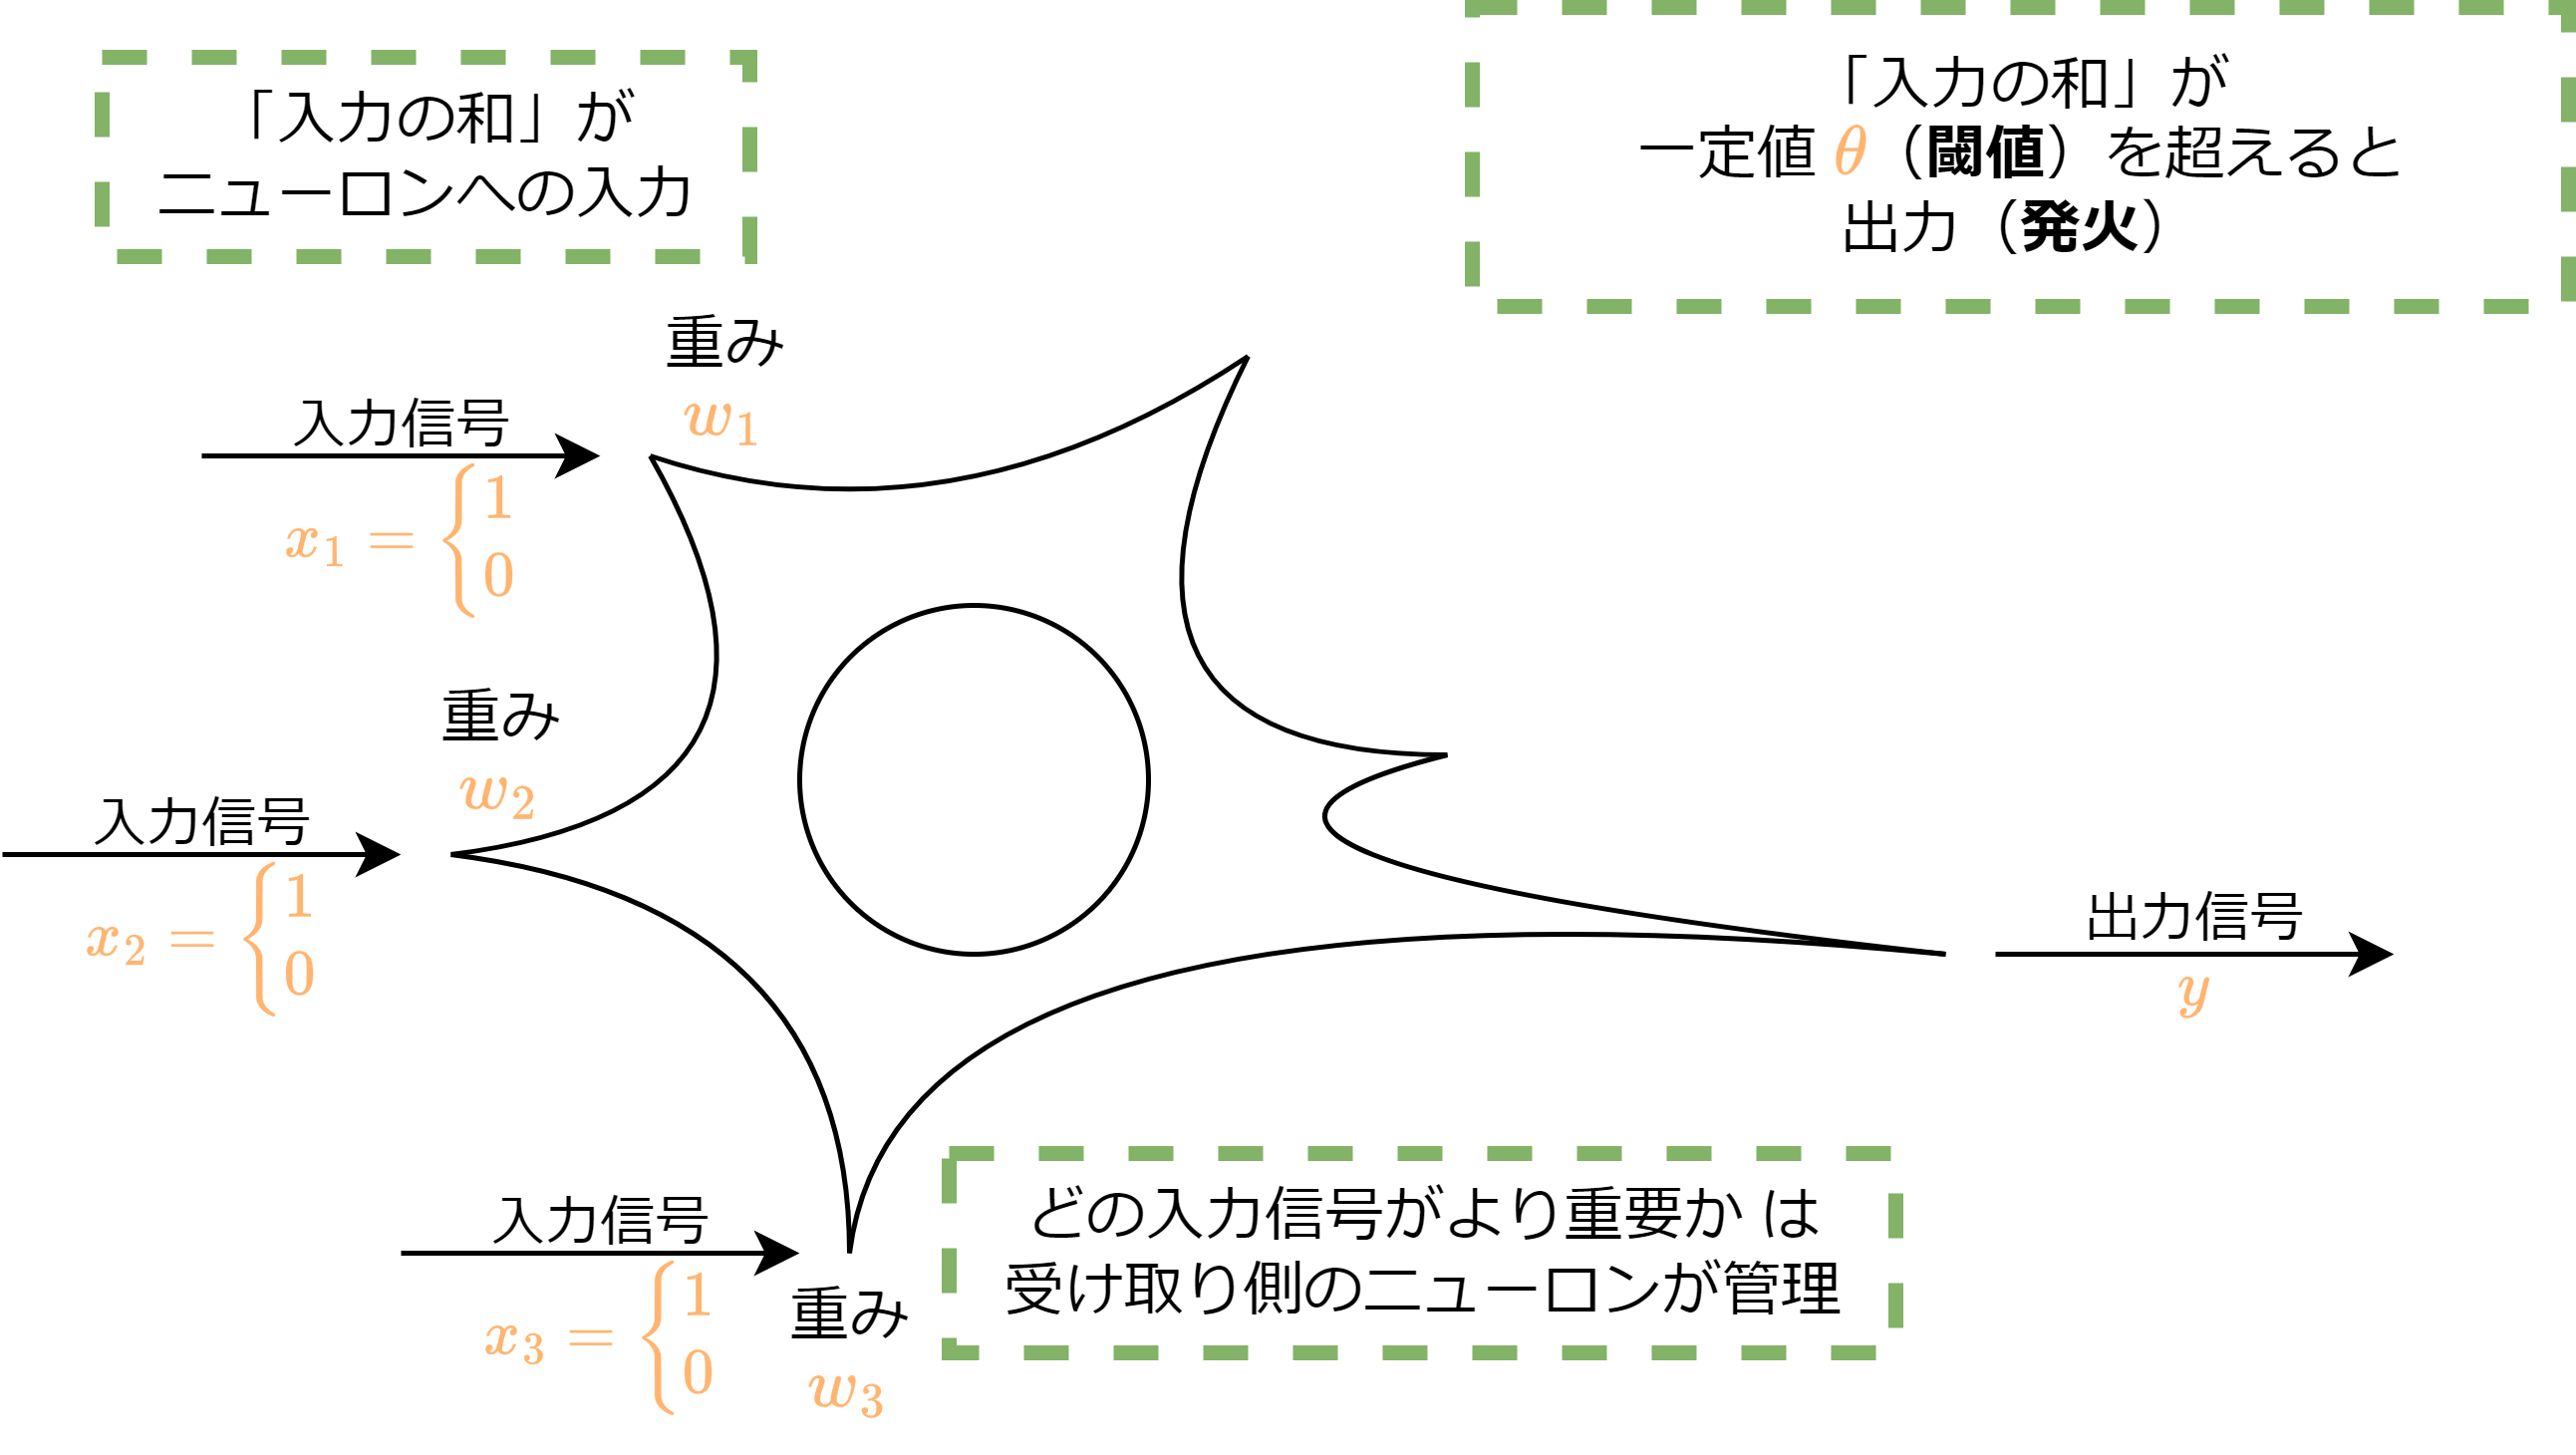
\includegraphics[width=0.7\linewidth]{img/mathematical-interpretation-of-neurons}
		\end{figure}
		\begin{itemize}
			\item 出力信号なし($ y = 0 $):$ w_1x_1 + w_2x_2 + w_3x_3 < \theta $
			\item 出力信号あり($ y = 1 $):$ w_1x_1 + w_2x_2 + w_3x_3 \geq \theta $
		\end{itemize}
	\end{frame}
	\begin{frame}{発火の条件のグラフ表現}
		\begin{figure}
			\centering
			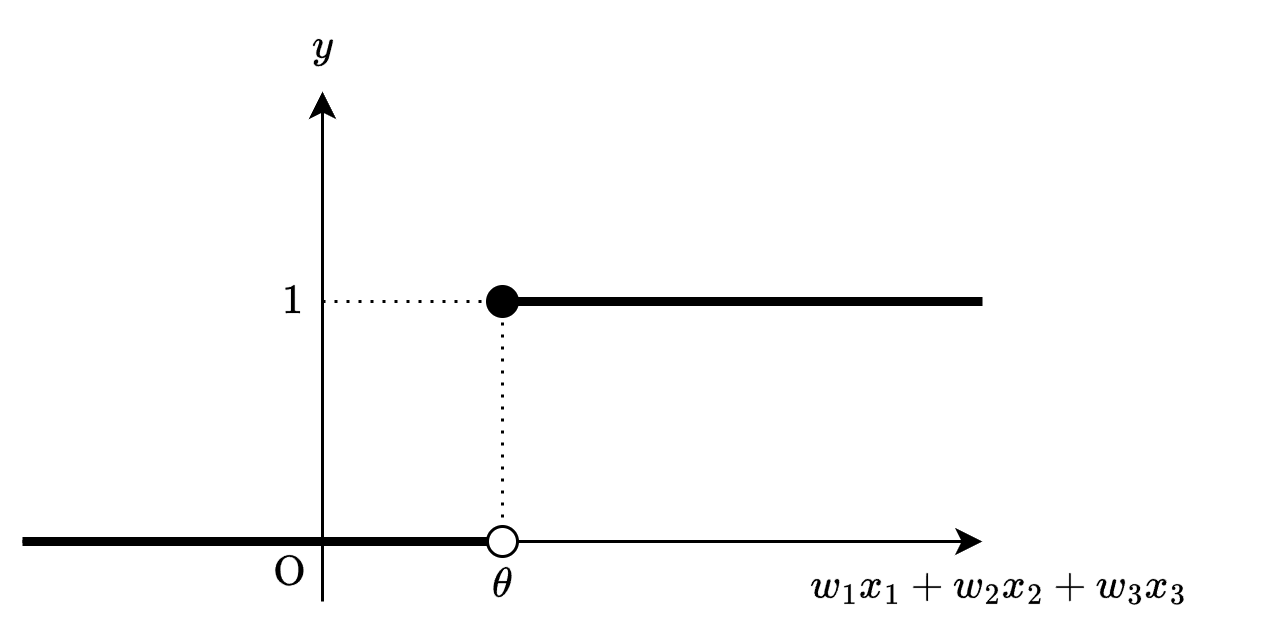
\includegraphics[width=0.9\linewidth]{img/graph-of-ignition-conditions}
		\end{figure}
	\end{frame}
	\begin{frame}{発火の式}
		\begin{itemize}
			\item 単位ステップ関数
		\end{itemize}
		\begin{figure}
			\centering
			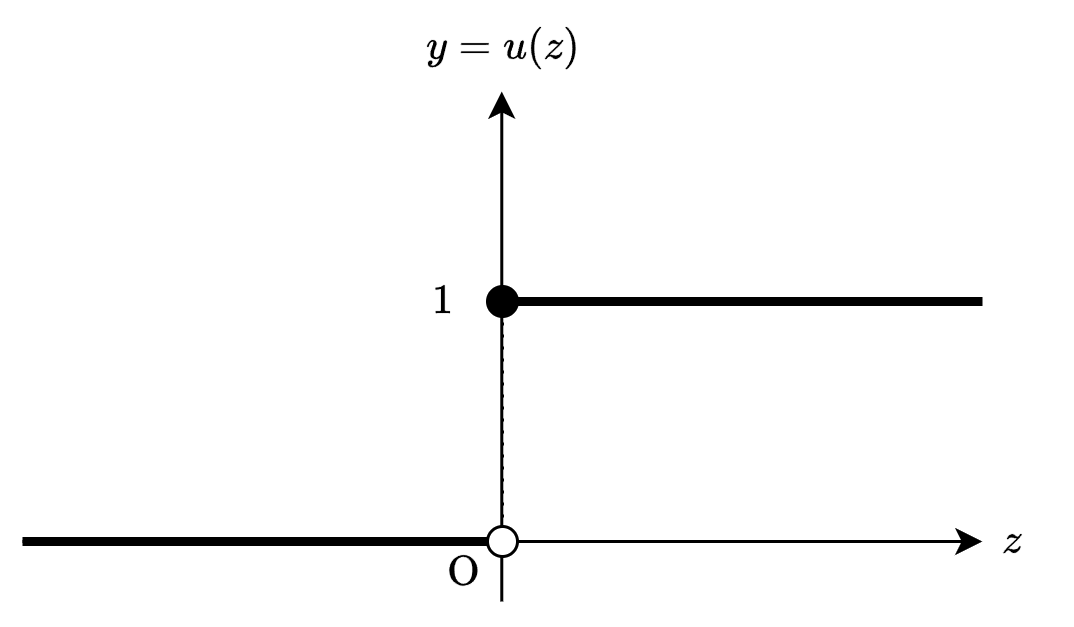
\includegraphics[width=0.5\linewidth]{img/unit-step-function}
		\end{figure}
		\begin{itemize}
			\item 発火の式:$ y = u(z) = u(w_1x_1 + w_2x_2 + w_3x_3 - \theta) $
			\begin{itemize}
				\item $ z = w_1x_1 + w_2x_2 + w_3x_3 - \theta $を、そのニューロンに対する\alert{重み付き入力}という
			\end{itemize}
		\end{itemize}
	\end{frame}
	\subsection{ユニット}
	\begin{frame}{ユニット}
		\begin{itemize}
			\item 簡略され抽象化されたニューロンを、生物学的なニューロンと区別して\alert{ユニット}(unit)とよぶ
		\end{itemize}
		\begin{figure}
			\centering
			
\includegraphics[width=0.7\linewidth]{img/unit}
		\end{figure}
	\end{frame}
	\begin{frame}{活性化関数}
		\begin{itemize}
			\item 発火の式(旧):$ y = u(w_1x_1 + w_2x_2 + w_3x_3 - \theta) $
			\begin{itemize}
				\item 単位ステップ関数$ u $に限定する必要はない
			\end{itemize}
			\item \alert{発火の式(新)}:$ y = a(w_1x_1 + w_2x_2 + w_3x_3 - \theta) $
			\begin{itemize}
				\item 関数$ a $を\alert{活性化関数}(activation function)という
				\item この関数$ a $はモデル作成者がさまざまに定義可能
			\end{itemize}
		\end{itemize}
	\end{frame}
	\begin{frame}{活性化関数の代表例}
		\alert{シグモイド関数}(Sigmoid function)
		\begin{equation*}
			\sigma(z) \triangleq \dfrac{1}{1 + e^{-z}}\quad (e = 2.71828\cdots)
		\end{equation*}
		\begin{figure}
			\centering
			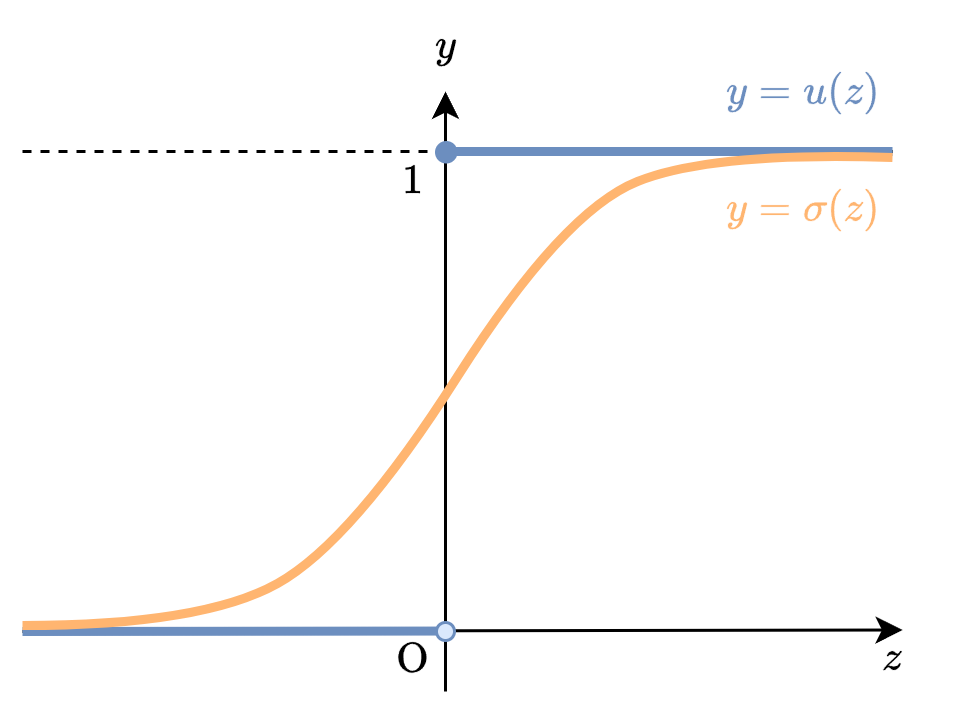
\includegraphics[width=0.5\linewidth]{img/unit-step-function-and-sigmoid-function}
		\end{figure}
	\end{frame}
	\begin{frame}{「発火の有無」から「興奮度」へ}
		\begin{figure}
			\centering
			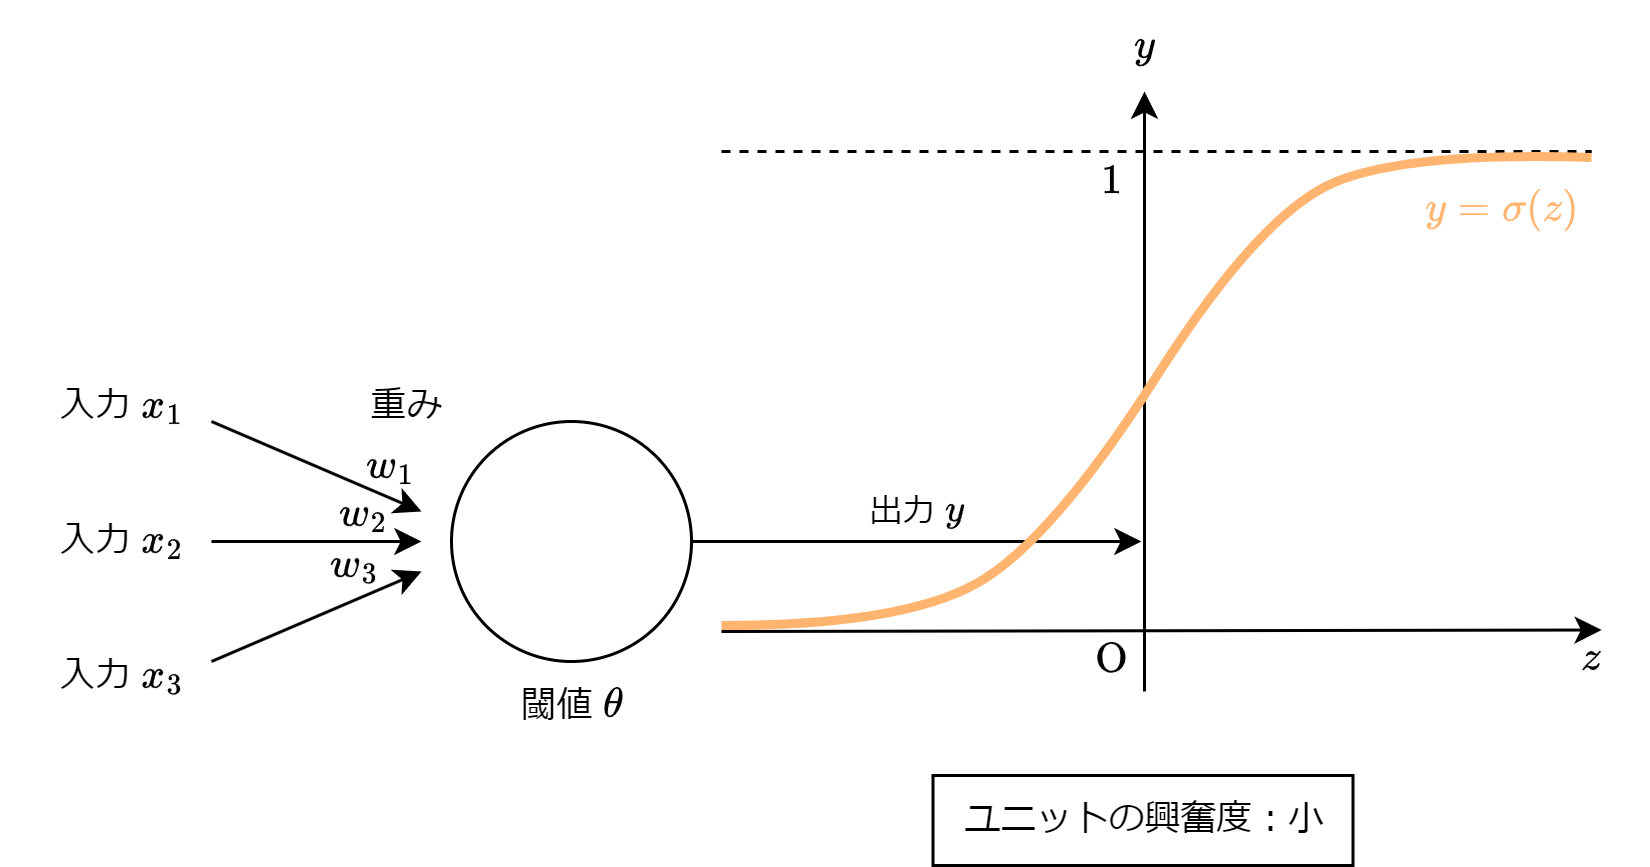
\includegraphics[width=0.8\linewidth]{img/unit-excitement-low}
		\end{figure}
		\begin{equation*}
			y = \sigma(w_1x_1 + w_2x_2 + w_3x_3 - \theta) 
		\end{equation*}
	\end{frame}
	\begin{frame}{「発火の有無」から「興奮度」へ}
		\begin{figure}
			\centering
			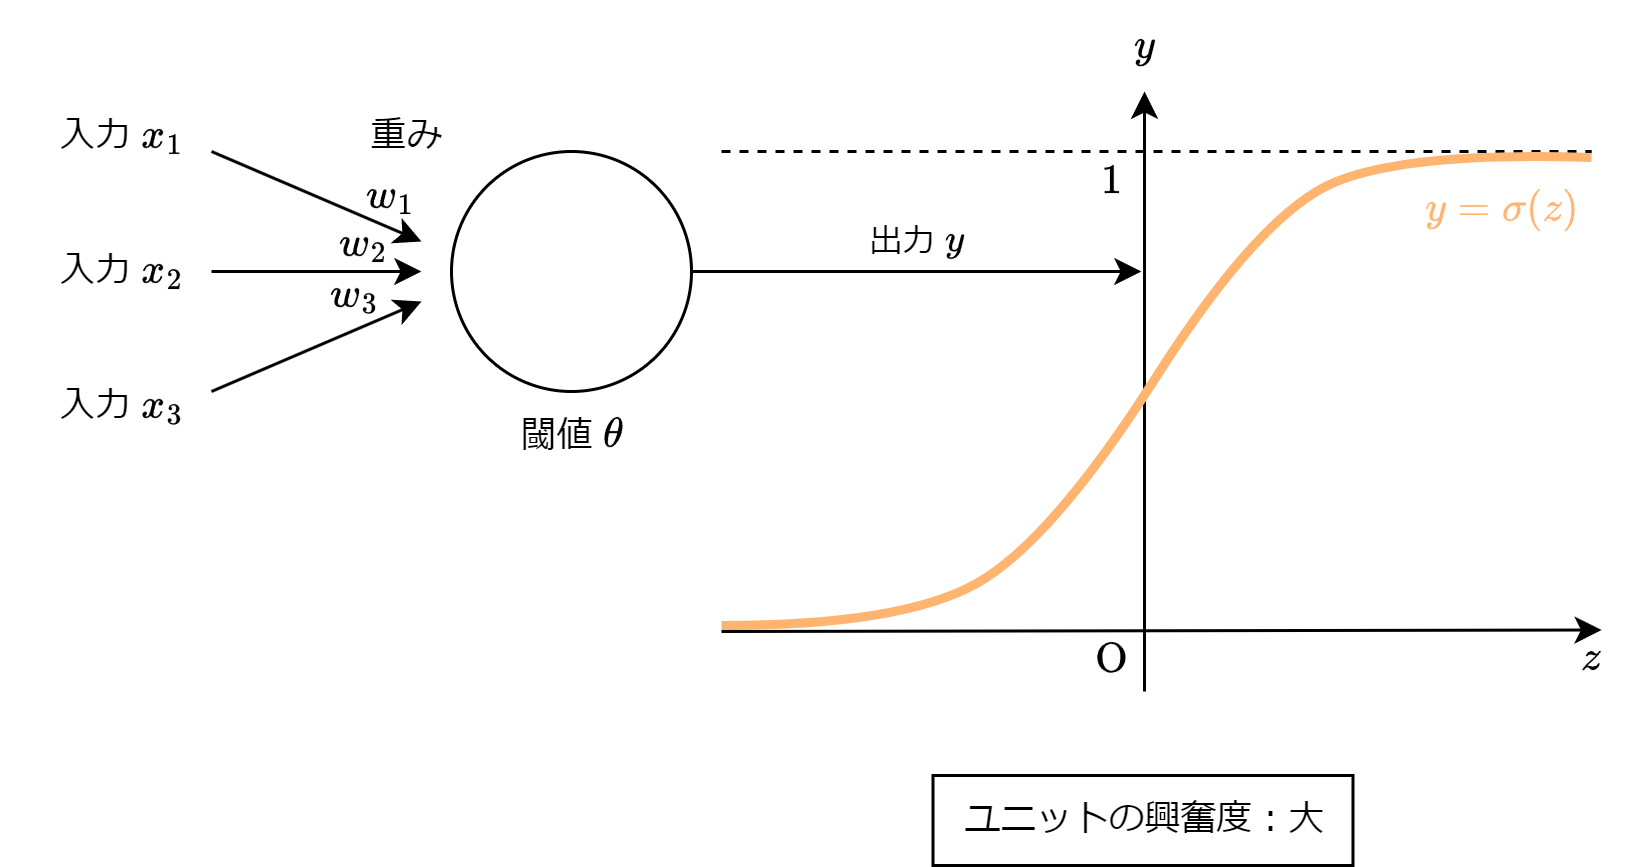
\includegraphics[width=0.8\linewidth]{img/unit-excitement-high}
		\end{figure}
		\begin{equation*}
			y = \sigma(w_1x_1 + w_2x_2 + w_3x_3 - \theta) 
		\end{equation*}
	\end{frame}
	\begin{frame}{バイアス}
		\sout{$ y = a(w_1x_1 + w_2x_2 + w_3x_3 - \theta) $}
		
		$ y = a(w_1x_1 + w_2x_2 + w_3x_3 + b) $		
		\begin{itemize}
			\item $ -\theta \longrightarrow +b $に表記を変更
			\item すべて足し算に統一することで計算しやすくなる
		\end{itemize}
	\end{frame}
	\begin{frame}{ユニットのまとめ}
		\begin{figure}
			\centering
			
\includegraphics[width=0.8\linewidth]{img/summary-of-unit}
		\end{figure}
		重み付き入力:$ z = w_1x_1 + w_2x_2 \cdots + w_nx_n + b $
		
		出力:$ y = \sigma(z) $
	\end{frame}

	\subsection{ニューラルネットワーク}
	\begin{frame}{ニューラルネットワーク(Neural Network; NN)}
		\begin{itemize}
			\item ユニットをネットワーク状に結合したもの
		\end{itemize}
		\begin{figure}
			\centering
			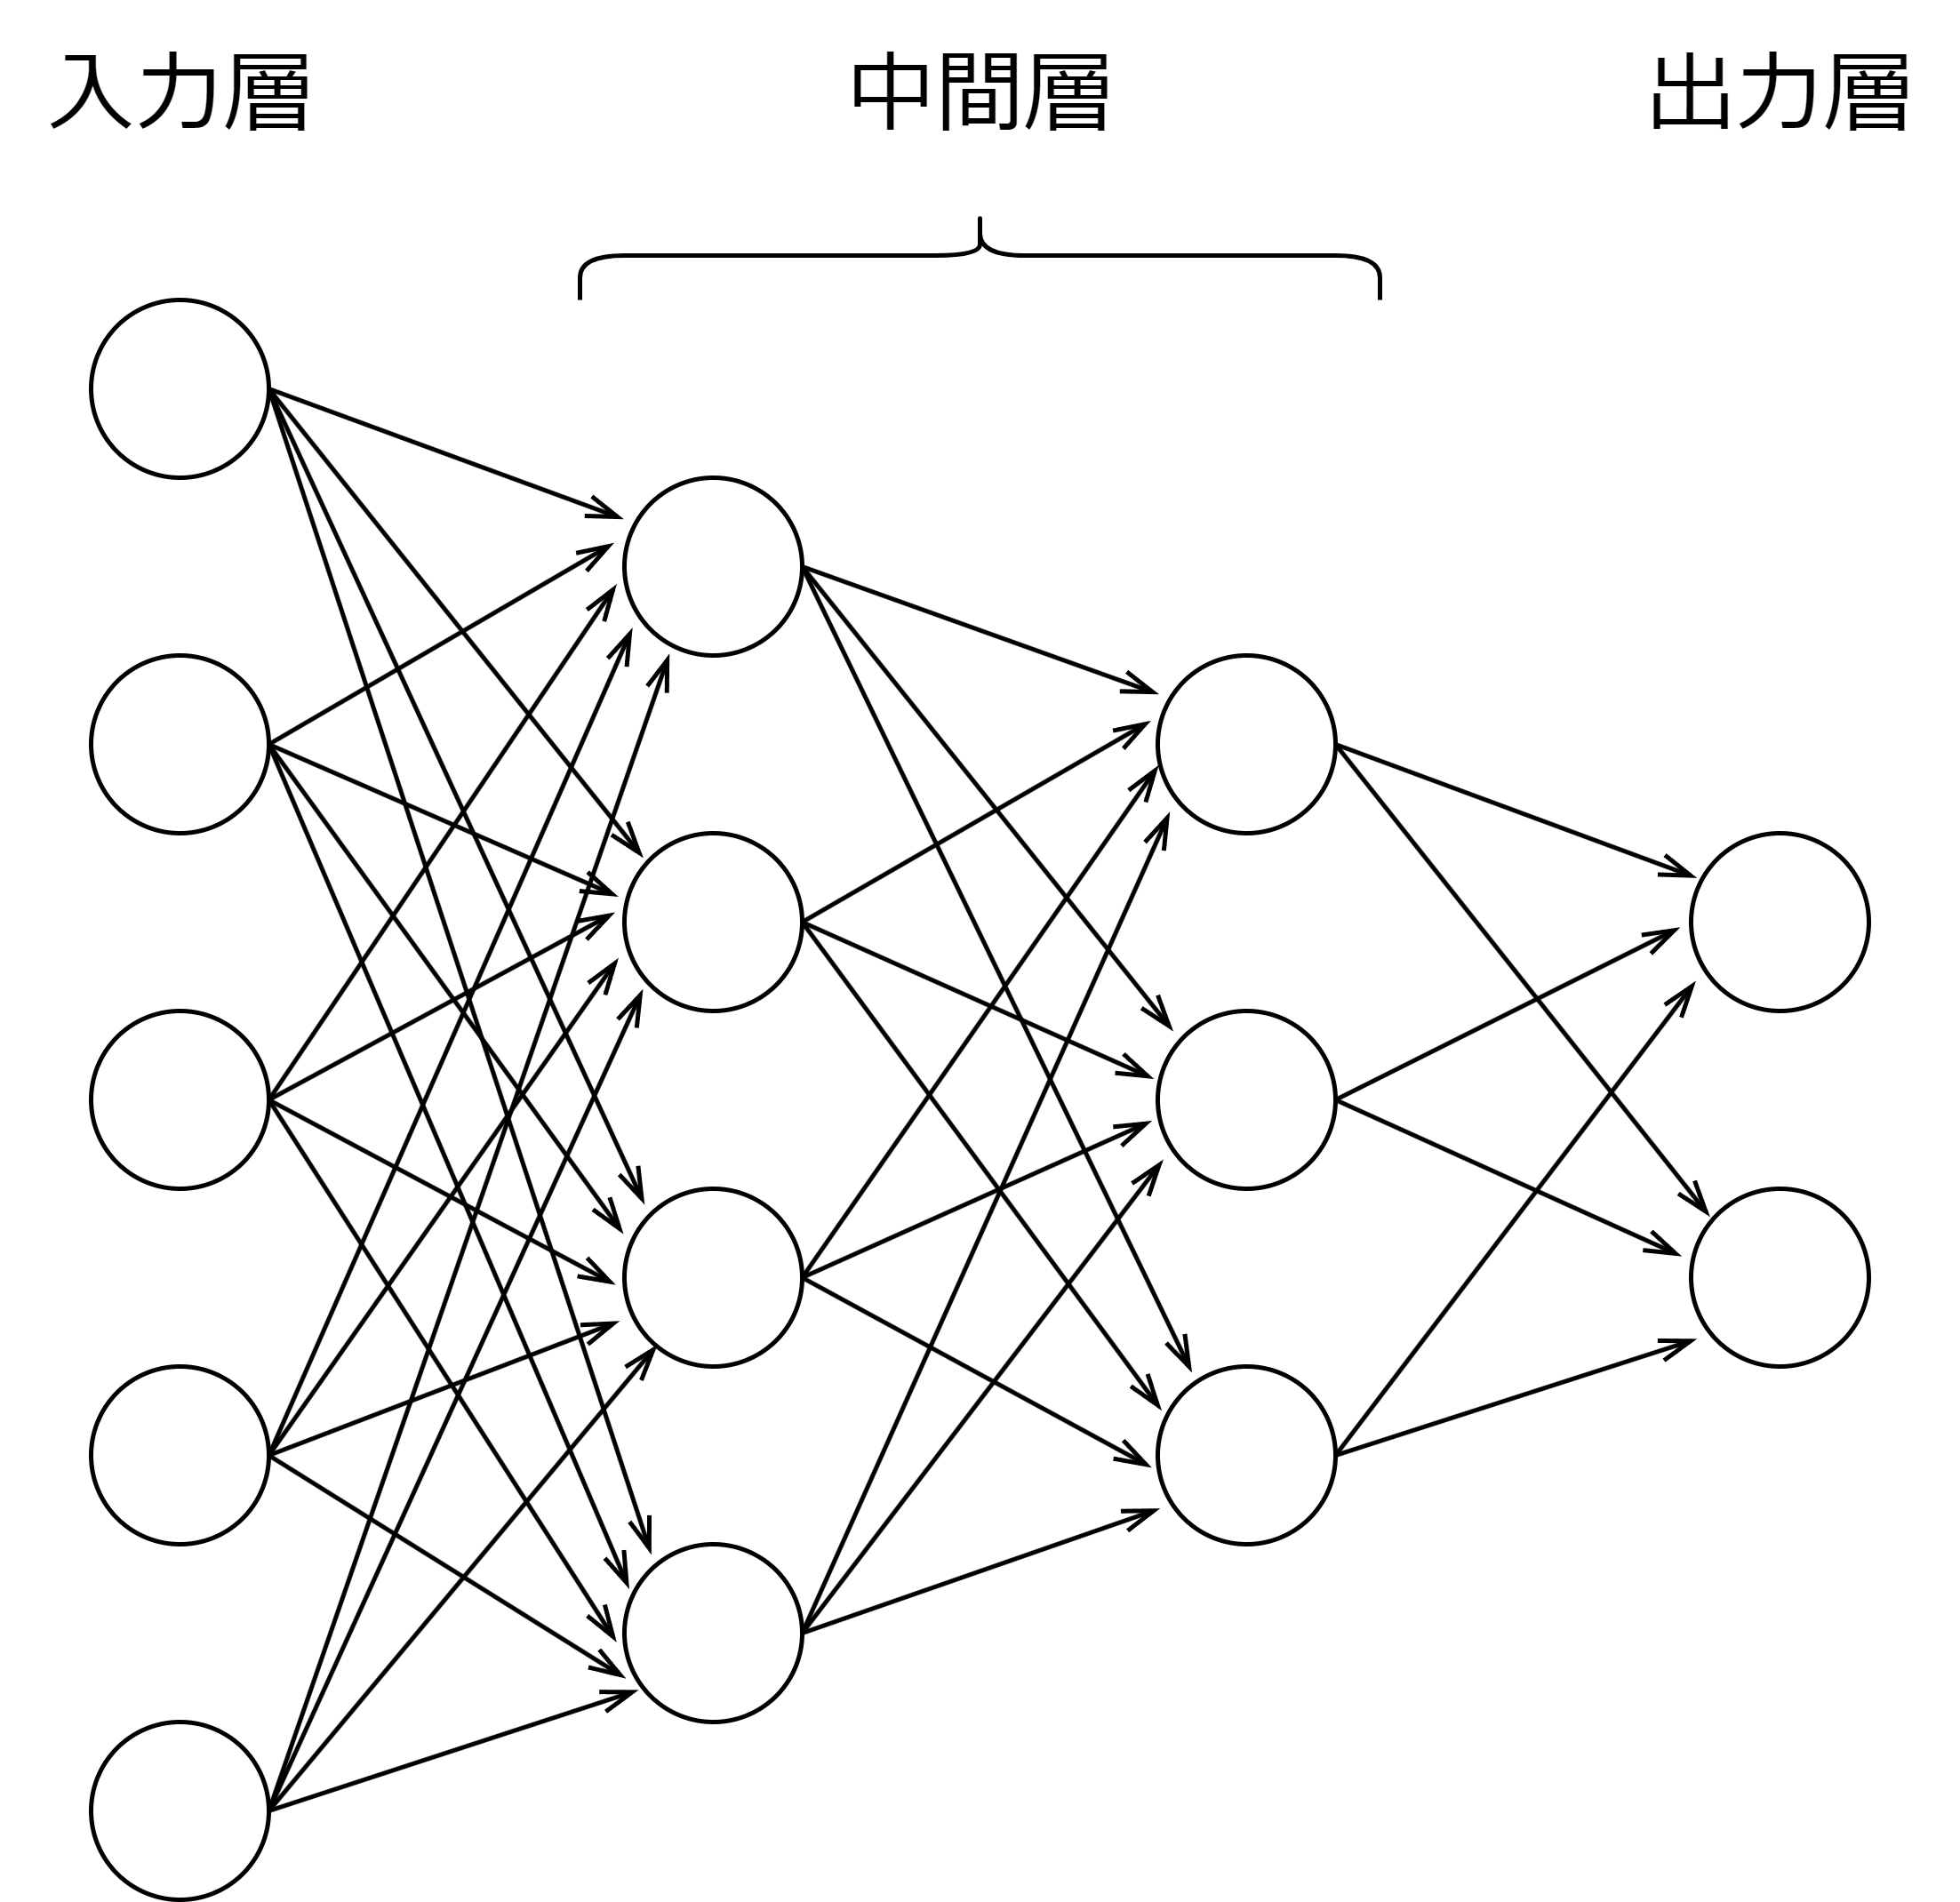
\includegraphics[width=0.4\linewidth]{img/hierarchical-neural-network}
		\end{figure}
	\end{frame}
	\begin{frame}{ニューラルネットワークを用いた問題の具体例}
		\begin{block}{例題}
			$ 4 \times 3 $画素からなる画像で読み取られた手書きの数字「0」「1」を識別するニューラルネットワークを作成せよ。
			ただし、学習データは64枚の画像とし、画素はモノクロ2階調とする。
		\end{block}
		\begin{figure}
			\centering
			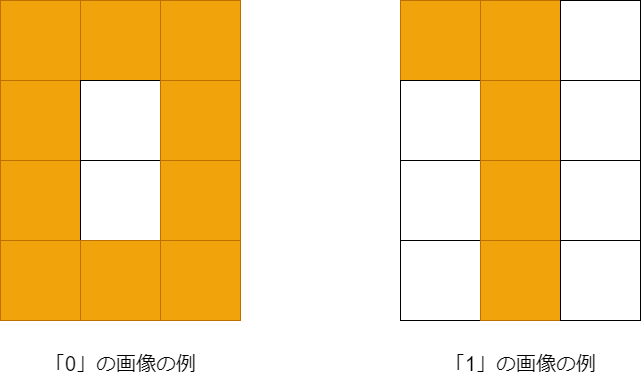
\includegraphics[width=0.5\linewidth]{img/examples-of-0-and-1-images}
		\end{figure}
	\end{frame}
	\begin{frame}{ニューラルネットワークを用いた問題の具体例}
		\underline{解答例}
		\begin{figure}
			\centering
			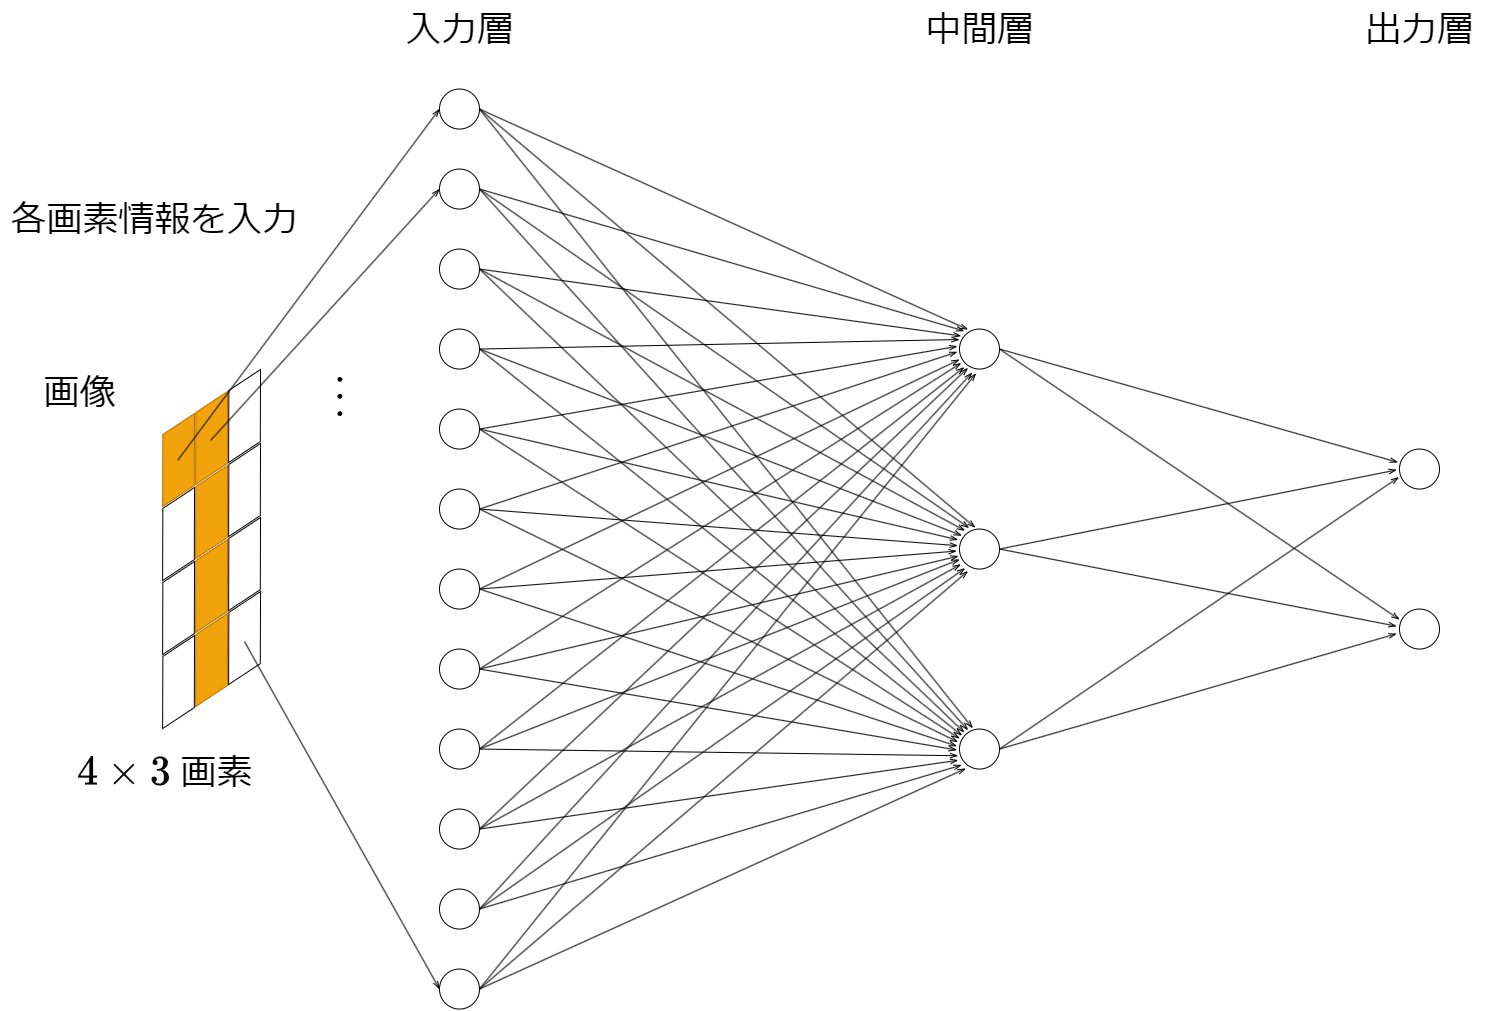
\includegraphics[width=0.6\linewidth]{img/examples-of-specific-neural-network-solutions}
		\end{figure}
	\end{frame}
	\begin{frame}{ニューラルネットワークの反応例}
		\begin{figure}
			\centering
			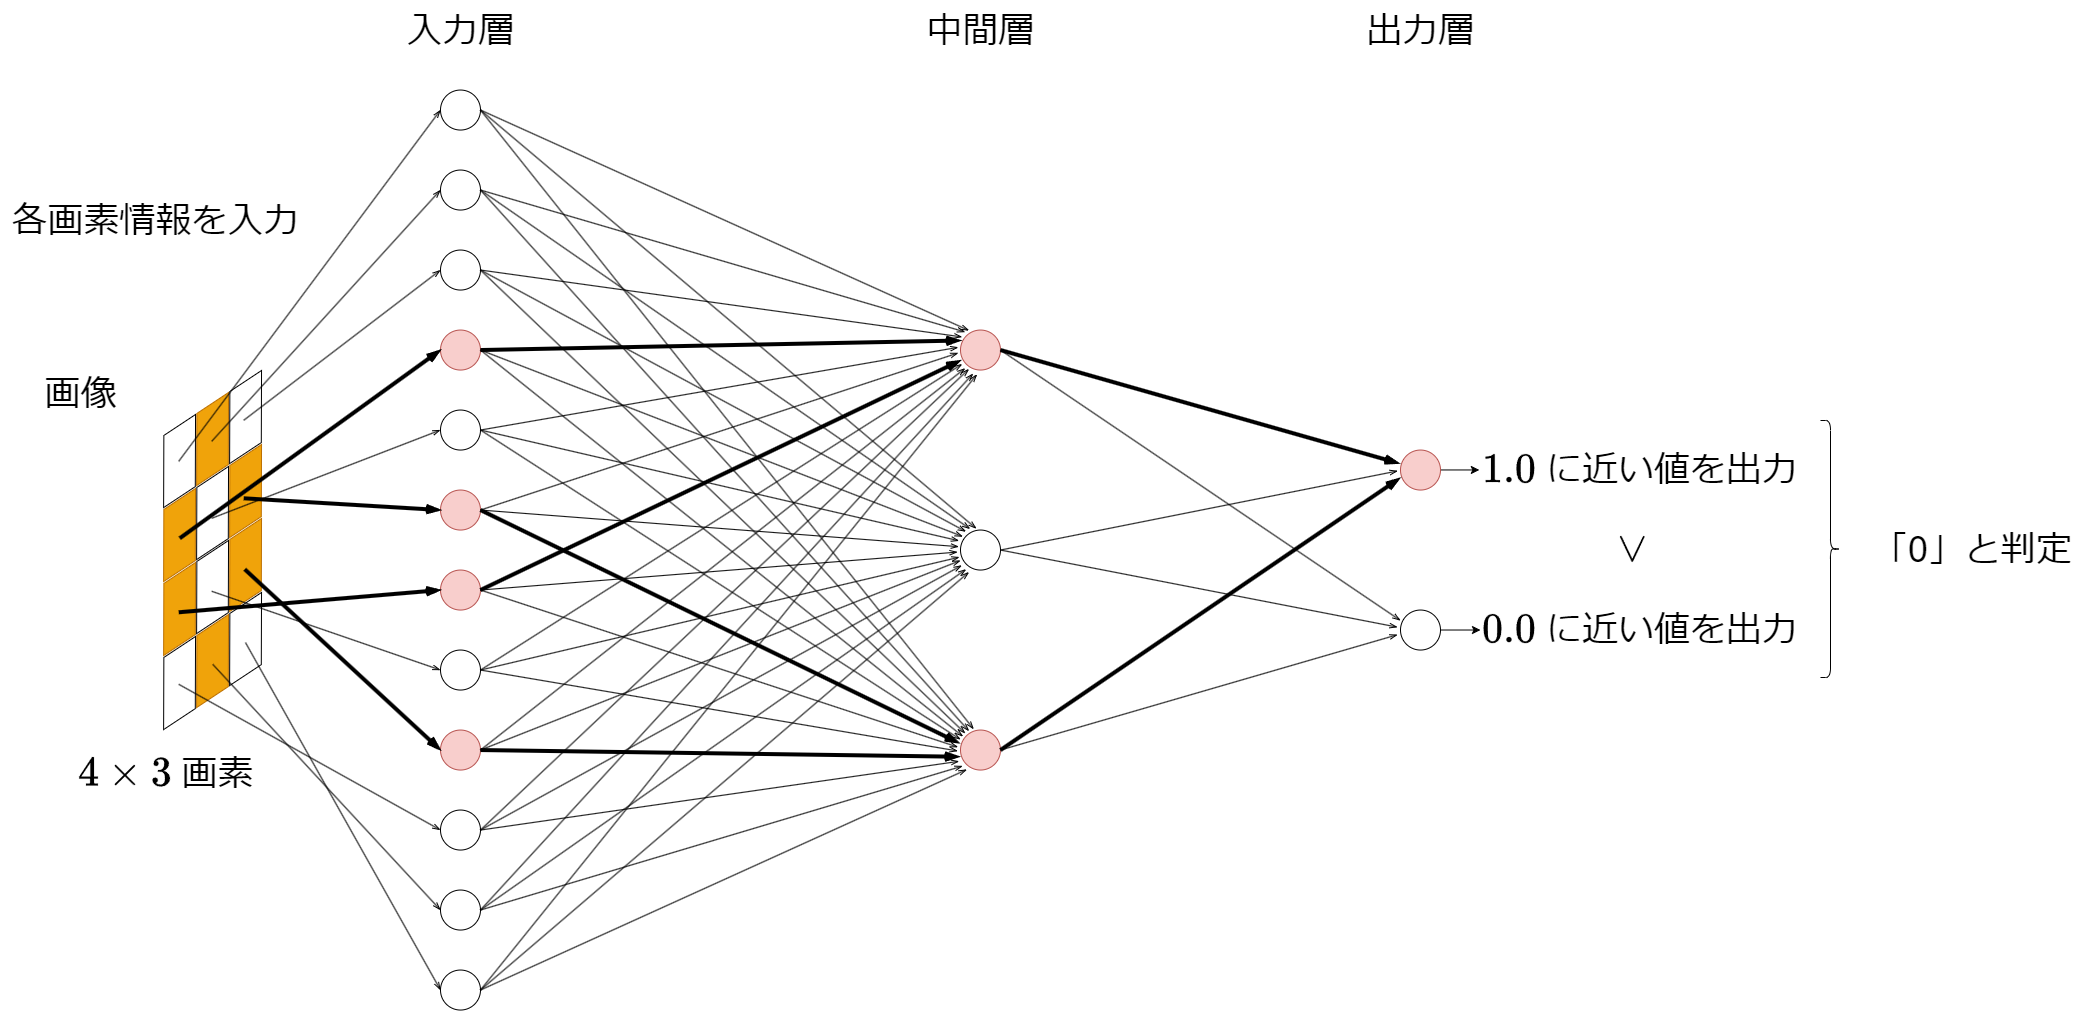
\includegraphics[width=0.7\linewidth]{img/example-of-response-of-neural-network-when-0-is-input}
		\end{figure}
	\end{frame}
	\begin{frame}{ニューラルネットワークの反応例}
		\begin{figure}
			\centering
			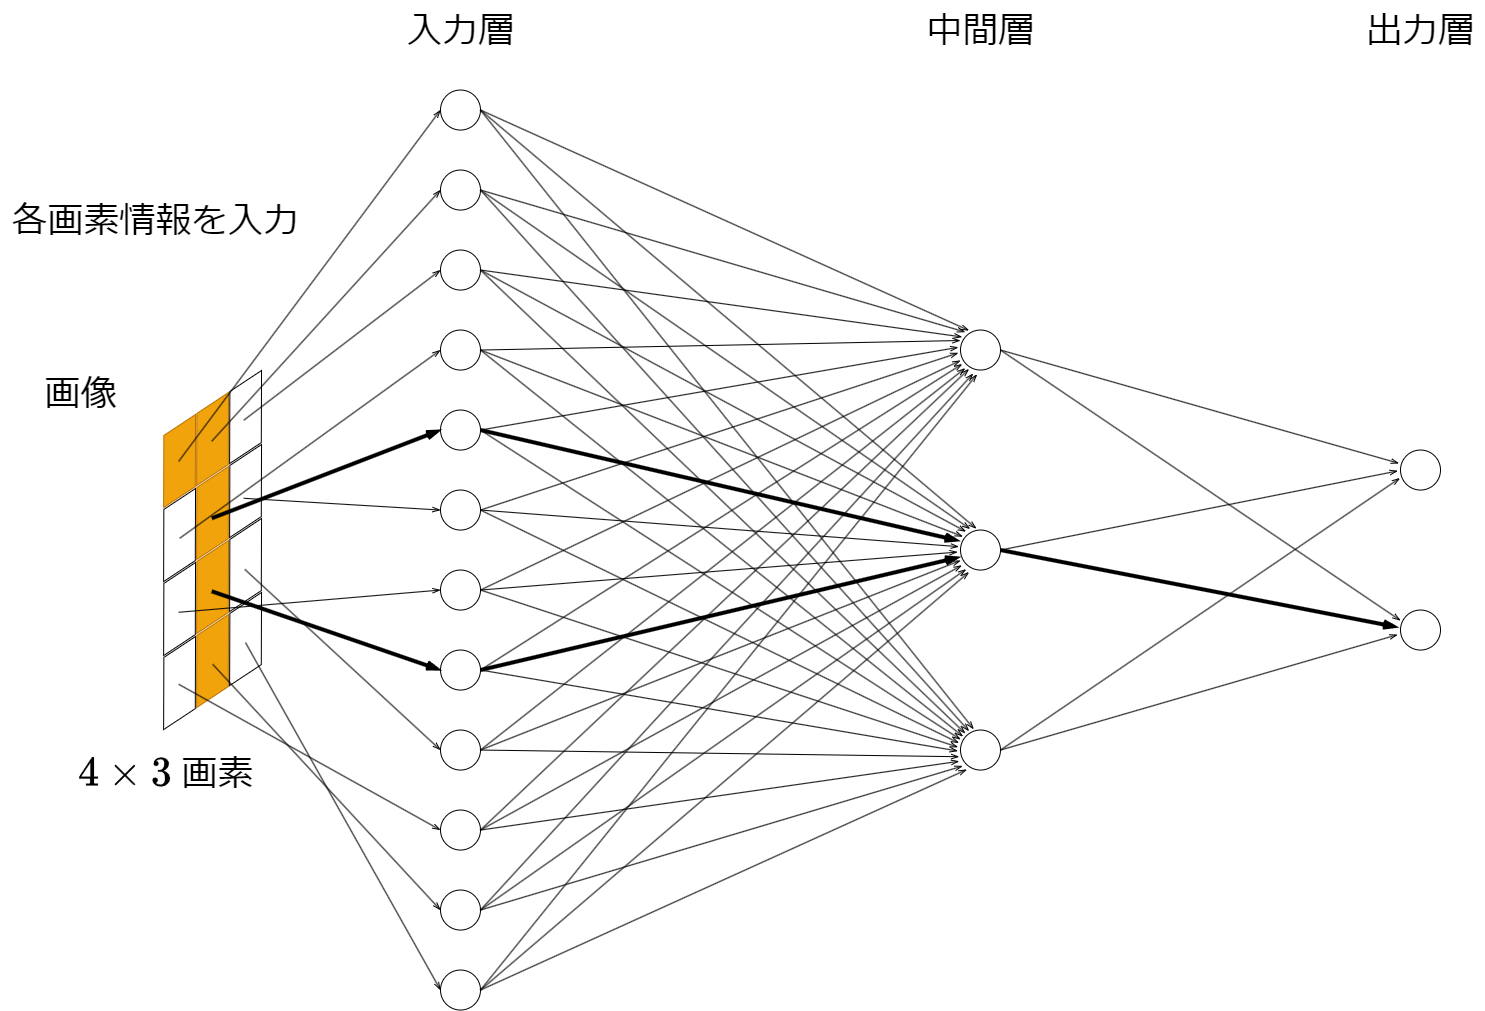
\includegraphics[width=0.7\linewidth]{img/example-of-response-of-neural-network-when-1-is-input}
		\end{figure}
	\end{frame}
	
	\section{数学の基礎}
	\subsection{ニューラルネットワークのための数学}

	\subsubsection{数列と漸化式}
	\begin{frame}{数列の意味}
		\begin{itemize}
			\item \alert{数列}:数の列
			\begin{itemize}
				\item \alert{項}:並べられたひとつひとつの数
				\item \alert{初項}:1番目の項
				\item \alert{第$ n $項}:$ n $番目の項
				\item \alert{有限数列}:有限個の項数を持つ数列
				\item \alert{末項}:有限数列において、数列の最後の項
				\item \alert{一般項}:数列の$ n $番目にある数で、通常$ a_n $などと表現する
			\end{itemize}
		\end{itemize}
		ニューラルネットワークにおいて、ユニットの重み付き入力やその出力は数列と考えられる
		
		\underline{例} $ a^l_j $:$ l $層$ j $番目のユニットの出力値
	\end{frame}
	\begin{frame}{数列と漸化式}
		\begin{itemize}
			\item \alert{漸化式}:初項$ a_1 $と、隣り合う2つの項$ a_n $, $ a_{n+1} $の関係式
			\item \alert{連立漸化式}:複数の数列がいくつかの関係式で結び付けられているもの
			\begin{itemize}
				\item ニューラルネットワークにおいて、ユニットの入力と出力は連立漸化式で結ばれている
			\end{itemize}
		\end{itemize}
		\begin{columns}
			\begin{column}{0.1\linewidth}
			\end{column}
			\begin{column}{0.4\linewidth}
				\begin{figure}
					\centering
					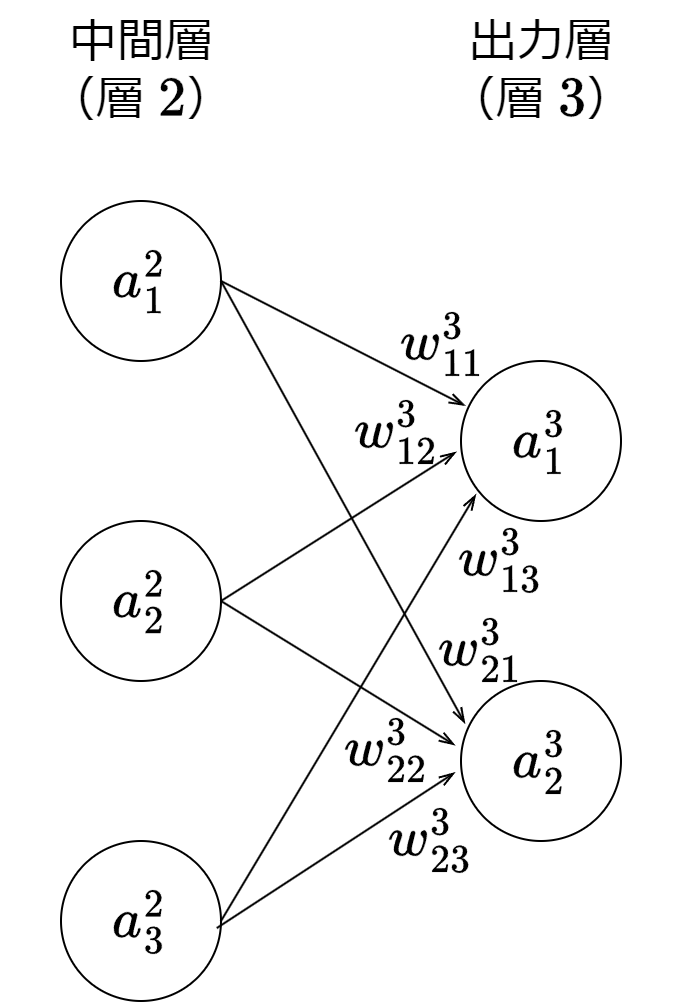
\includegraphics[width=0.5\linewidth]{img/example-of-simultaneous-asymptotic-formulas}
				\end{figure}
			\end{column}
			\begin{column}{0.5\linewidth}
				$ a^3_1 = \sigma(w^3_{11}a^2_1 + w^3_{12}a^2_2 + w^3_{13}a^2_3 + b^3_1) $\\
				$ a^3_2 = \sigma(w^3_{21}a^2_1 + w^3_{22}a^2_2 + w^3_{23}a^2_3 + b^3_2) $
			\end{column}
		\end{columns}
	\end{frame}

	\subsubsection{$ \sum $記号}
	\begin{frame}{$ \sum $記号の意味}
		\underline{公式}
		\begin{enumerate}
			\item[(I)]  $ \displaystyle\sum_{k=1}^n a_k = a_1 + a_2 + \cdots + a_{n-1} + a_n $
			\item[(II)] $ \displaystyle\sum_{k=1}^n (a_k + b_k) = \sum_{k=1}^n a_k + \sum_{k=1}^n b_k $
			\item[(III)] $ \displaystyle\sum_{k=1}^n ca_k = c\sum_{k=1}^n a_k $($ c $:定数)
		\end{enumerate}
	\end{frame}

	\subsubsection{ベクトル}
	\begin{frame}{有向線分とベクトル}
		\begin{columns}
			\begin{column}{0.5\linewidth}
				\begin{itemize}
					\item \alert{有向線分}:向きを持つ線分
					\begin{itemize}
						\item (始点の)\alert{位置}
						\item (線分の始点から終点への)\alert{向き}
						\item (線分の)\alert{大きさ}
					\end{itemize}
					\item \alert{ベクトル}:有向線分から位置の属性を抜いたもの
					\begin{itemize}
						\item (線分の始点から終点への)\alert{向き}
						\item (線分の)\alert{大きさ}
					\end{itemize}
				\end{itemize}
			\end{column}
			\begin{column}{0.5\linewidth}
				\begin{figure}
					\centering
					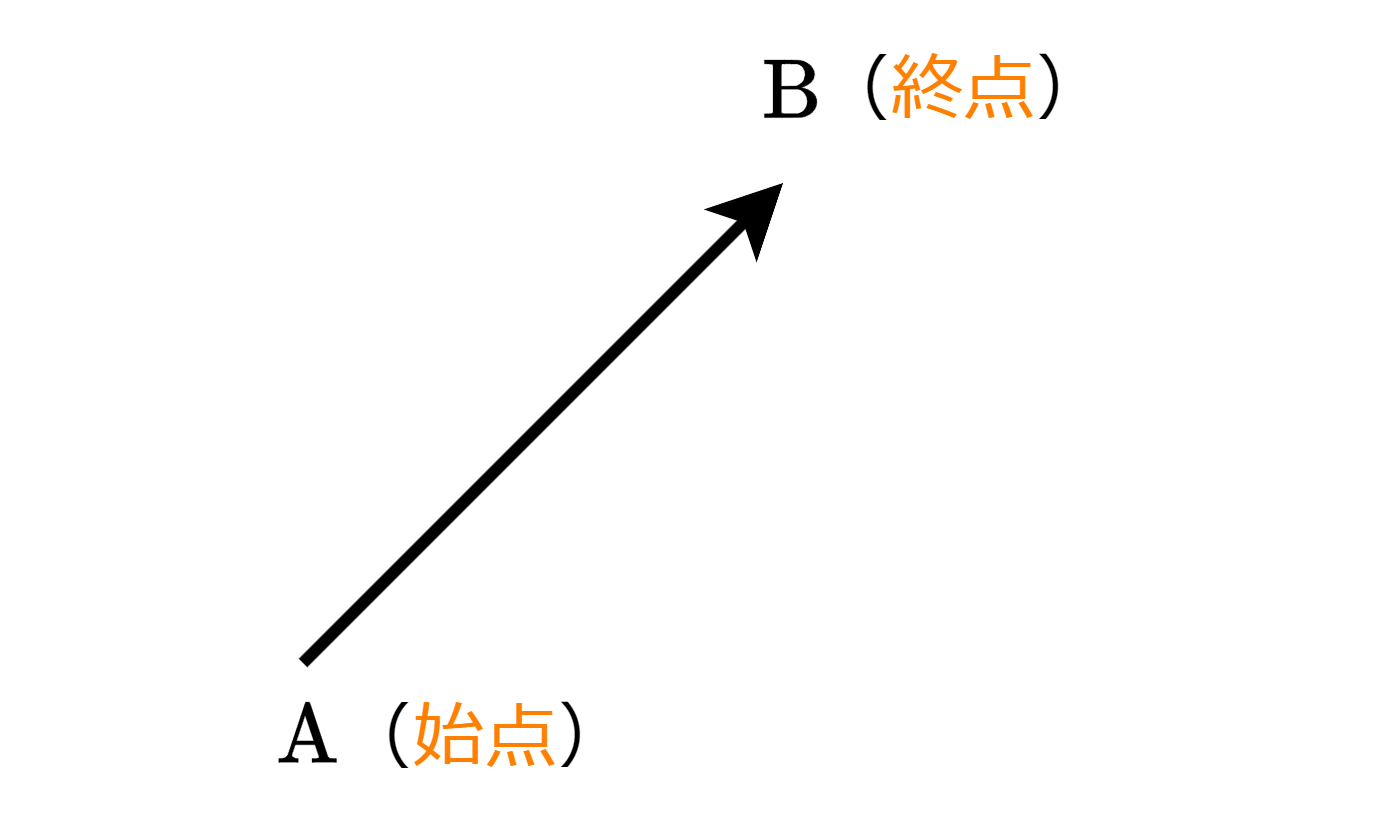
\includegraphics[width=0.9\linewidth]{img/directed-line-segment-and-vector}
				\end{figure}
			\end{column}
		\end{columns}
	\end{frame}
	\begin{frame}{ベクトルの成分表示}
		\begin{figure}
			\centering
			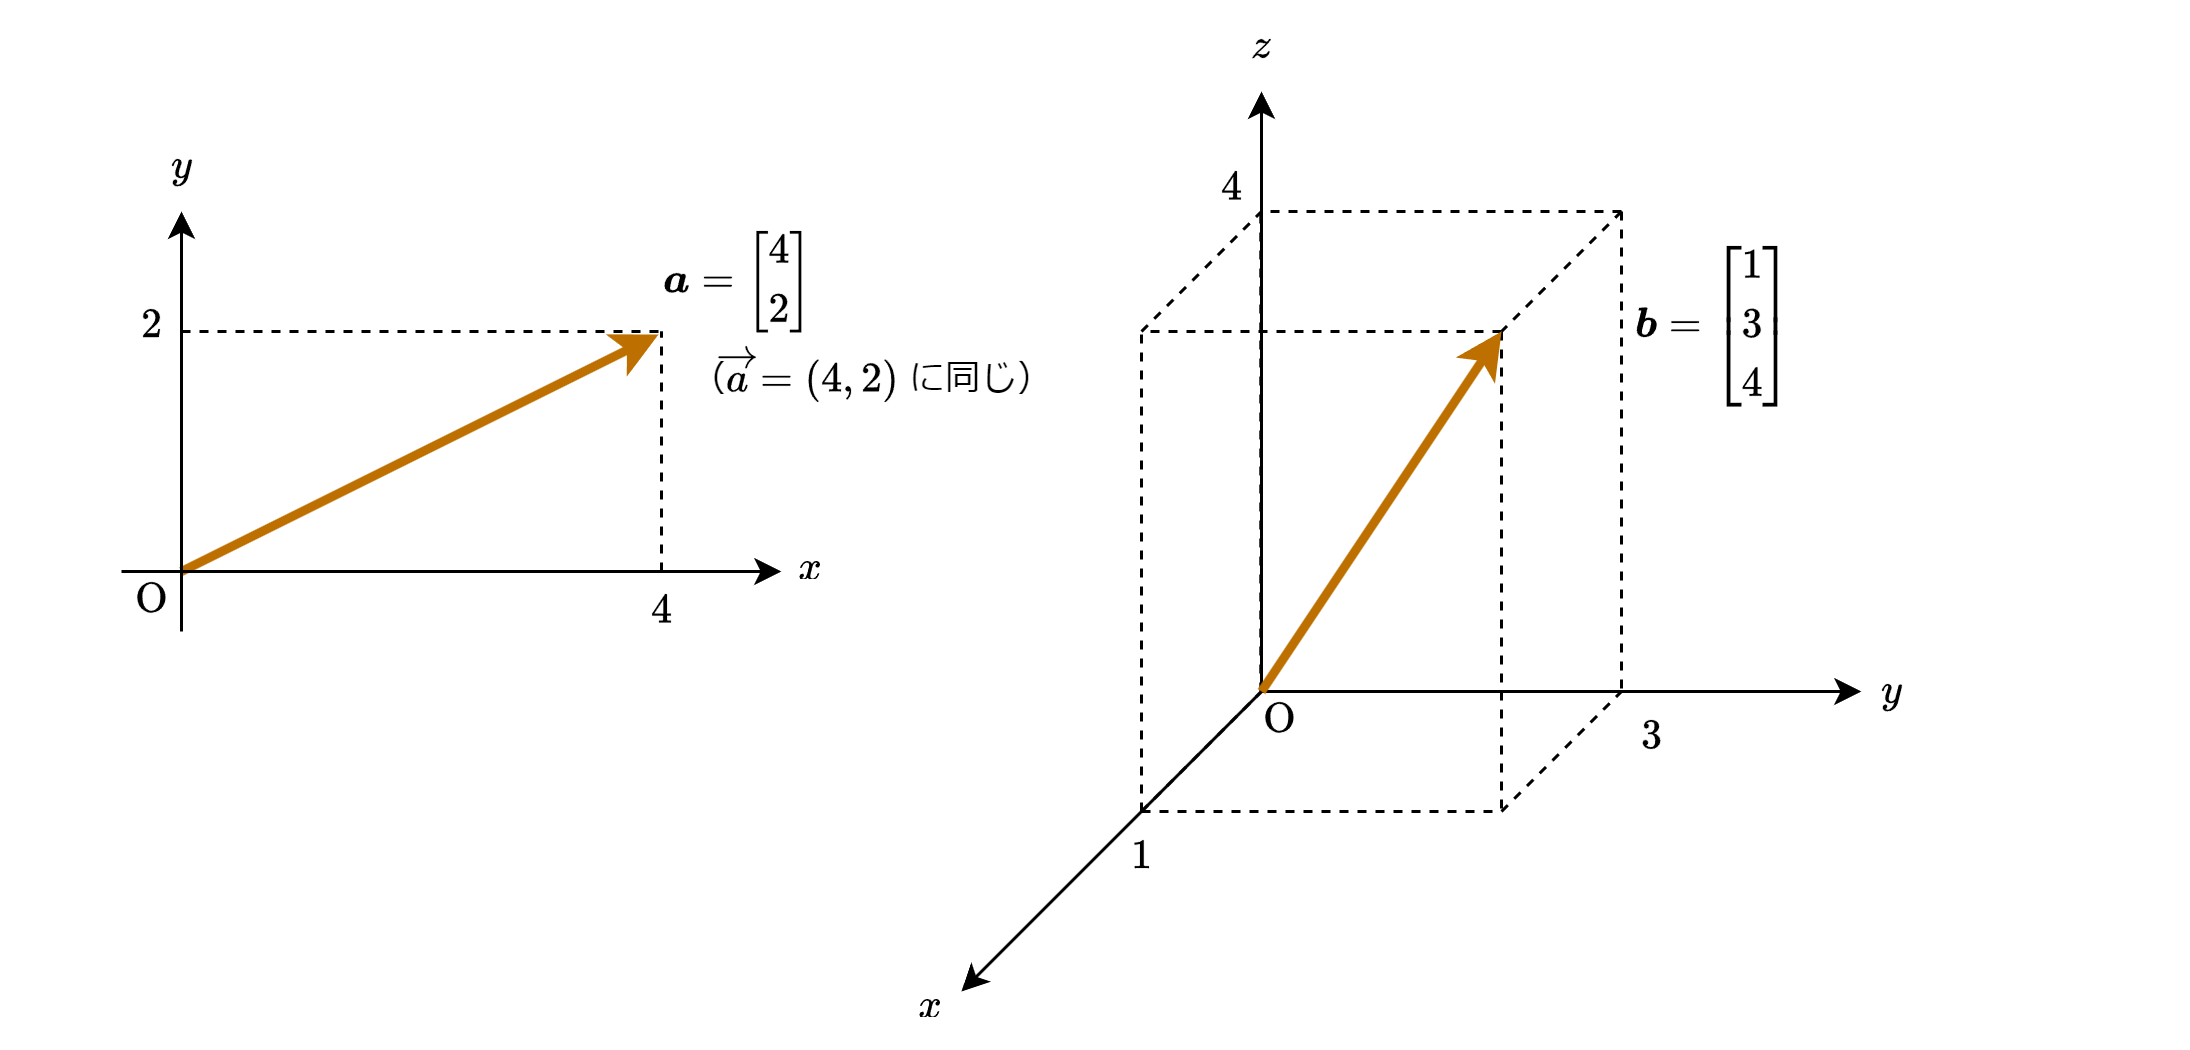
\includegraphics[width=0.9\linewidth]{img/component-display-of-vectors}
		\end{figure}
	\end{frame}
	\begin{frame}{ベクトルの基本公式}
		\underline{ベクトル$ \boldsymbol{a} $の大きさ$ \|\boldsymbol{a}\| $}
		
		$ \boldsymbol{a} = \begin{bmatrix}
			a_1\\
			\vdots\\
			a_n
		\end{bmatrix} $のとき、$ \|\boldsymbol{a}\| \triangleq \sqrt{a_1^2 + \cdots + a_n^2} = \sqrt{\displaystyle\sum_{k=1}^n a_k^2} \geq 0. $
	
		\underline{例} $ \boldsymbol{a} = \begin{bmatrix}
			-1\\
			2
		\end{bmatrix} $のとき、$ \|\boldsymbol{a}\| = \sqrt{(-1)^2 + 2^2} = 1 + 4 = 5. $
	\end{frame}
	\begin{frame}{ベクトルの基本公式}
		\underline{ベクトル$ \boldsymbol{a}, \boldsymbol{b} $の内積$ \langle\boldsymbol{a}, \boldsymbol{b} \rangle $}
		
		\begin{itemize}
			\item
				ベクトル$ \boldsymbol{a}, \boldsymbol{b} $のなす角を$ \theta $とすると、$ \langle\boldsymbol{a}, \boldsymbol{b} \rangle \triangleq \|\boldsymbol{a}\| \|\boldsymbol{b}\| \cos\theta. $
			\item
				$ \boldsymbol{a} = \begin{bmatrix}
					a_1\\
					\vdots\\
					a_n
				\end{bmatrix},\ \boldsymbol{b} = \begin{bmatrix}
					b_1\\
					\vdots\\
					b_n
				\end{bmatrix} $とすると、$ \langle\boldsymbol{a}, \boldsymbol{b} \rangle \triangleq a_1b_1 + a_2b_2 + \cdots + a_nb_n = \displaystyle\sum_{k=1}^n a_kb_k.$
		\end{itemize}
		
		\underline{例} $ \boldsymbol{a} = \begin{bmatrix}
			2\\
			3
		\end{bmatrix},\ \boldsymbol{b}= \begin{bmatrix}
			5\\
			1
		\end{bmatrix} $のとき、$ \langle\boldsymbol{a}, \boldsymbol{b}\rangle = 2\cdot5 + 3\cdot1 = 13. $
	\end{frame}
	\begin{frame}{ベクトルの基本公式}
		\underline{コーシー・シュワルツの不等式}
		
		ベクトル$ \boldsymbol{a}, \boldsymbol{b} $に対して、
		\begin{equation*}
			-\|\boldsymbol{a}\| \|\boldsymbol{b}\| \leq \langle\boldsymbol{a}, \boldsymbol{b}\rangle \leq \|\boldsymbol{a}\| \|\boldsymbol{b}\|
		\end{equation*}
		が成り立つ。
	\end{frame}
	\begin{frame}{コラム:ベクトルがどう役に立つ?}
		ニューラルネットワークの出力$ y $
		\begin{center}
			
\includegraphics[width=0.5\linewidth]{img/summary-of-unit}
		\end{center}
		$ y = \sigma(\highlight[red]{$ w_1x_1 + \cdots + w_nx_n $} +b) = \sigma\left(\highlight[red]{$ \left\langle\begin{bmatrix}
			w_1\\
			\vdots\\
			w_n
		\end{bmatrix},\ \begin{bmatrix}
			x_1\\
			\vdots\\
			x_n
		\end{bmatrix}\right\rangle $} + b\right) = \sigma(\highlight[red]{$ \langle\boldsymbol{w}, \boldsymbol{x}\rangle $} + b). $
	\end{frame}	
	
	\subsubsection{行列}
	\begin{frame}{行列とは}
		数を縦と横に矩形上に配列したもの
		% TODO: \usepackage{graphicx} required
		\begin{figure}
			\centering
			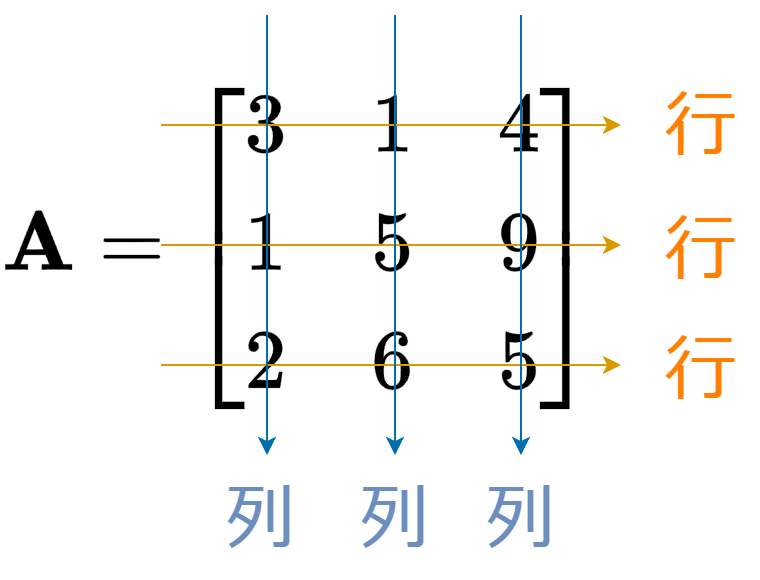
\includegraphics[width=0.4\linewidth]{img/example-of-matrix}
		\end{figure}
	\end{frame}
	\begin{frame}{ベクトルも行列の一部}
		$ \begin{bmatrix}
			x\\ y\\ z
		\end{bmatrix} $は3行1列の行列とみなせる
	\end{frame}
	\begin{frame}{行列同士の演算}
		行列の和
		
		$ \begin{bmatrix}
			a&b\\
			c&d
		\end{bmatrix} + \begin{bmatrix}
			p&q\\
			r&s
		\end{bmatrix} = \begin{bmatrix}
			a+p & b+q\\
			c+r & d+s
		\end{bmatrix} $
		
		行列の積
		
		$ \begin{bmatrix}
			a&b\\
			c&d
		\end{bmatrix}\begin{bmatrix}
			p&q\\
			r&s
		\end{bmatrix} = \begin{bmatrix}
			ap+br & aq+bs\\
			cp+dr & cq+ds
		\end{bmatrix} $
	
		% TODO: \usepackage{graphicx} required
		\begin{figure}
			\centering
			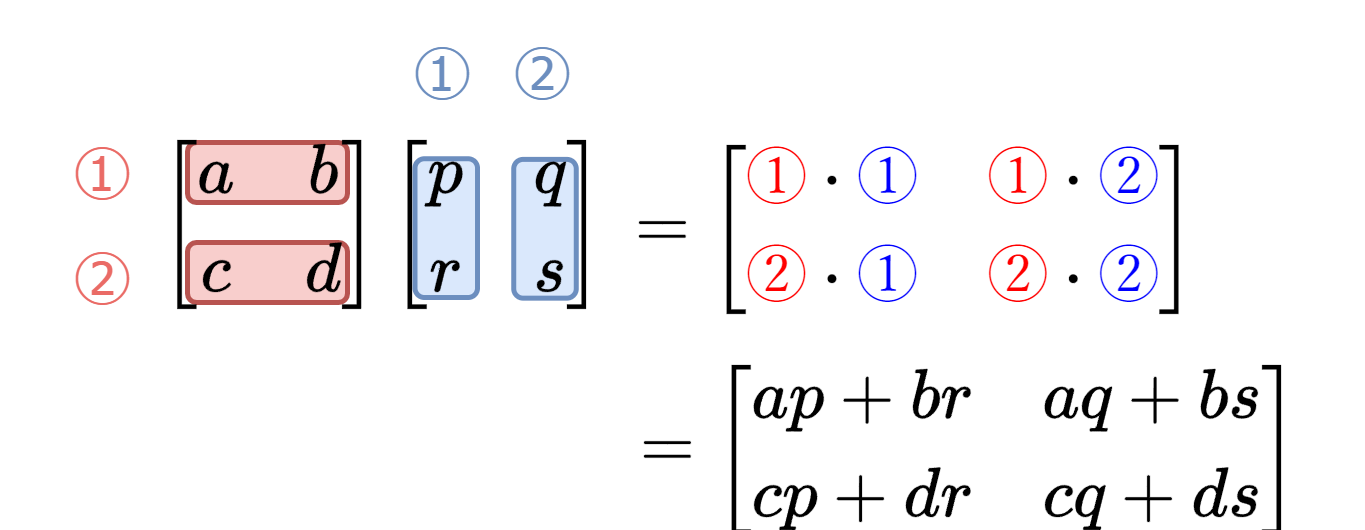
\includegraphics[width=0.5\linewidth]{img/product-of-matrices}
		\end{figure}
		
	\end{frame}
	\begin{frame}{行列とベクトルの演算}
		% TODO: \usepackage{graphicx} required
		\begin{figure}
			\centering
			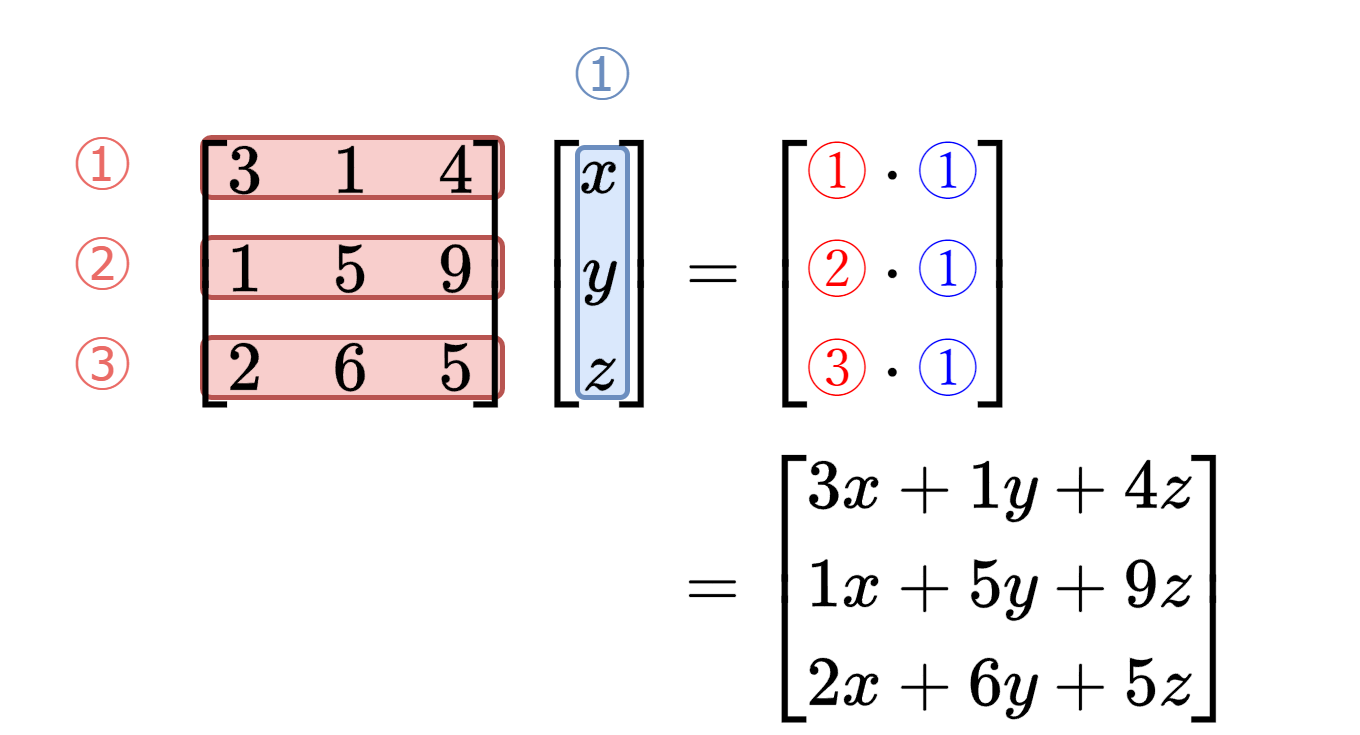
\includegraphics[width=0.6\linewidth]{img/product-of-matrix-and-vector}
		\end{figure}
		
	\end{frame}
	\subsection{勾配降下法のための数学}
	\subsubsection{微分}
	\begin{frame}{微分の定義}
		関数$ y=f(x) $対して\alert{導関数}$ f'(x) $は次のように定義される:
		\begin{equation*}
			f'(x) \triangleq \lim_{\Delta x \to 0} \dfrac{f(x + \Delta x) - f(x)}{\Delta x}.
		\end{equation*}
	
		※「$ \displaystyle\lim_{\Delta x \to 0} (\Delta x \text{の式}) $」は「数$ \Delta x $を限りなく$ 0 $に近づけたとき、$ (\Delta x \text{の式}) $の近づく値」を意味する
		
		関数$ f(x) $の導関数$ f'(x) $を求めることを「関数$ f(x) $を\alert{微分する}」という
	\end{frame}
	\begin{frame}{導関数の意味}
		\begin{figure}
			\centering
			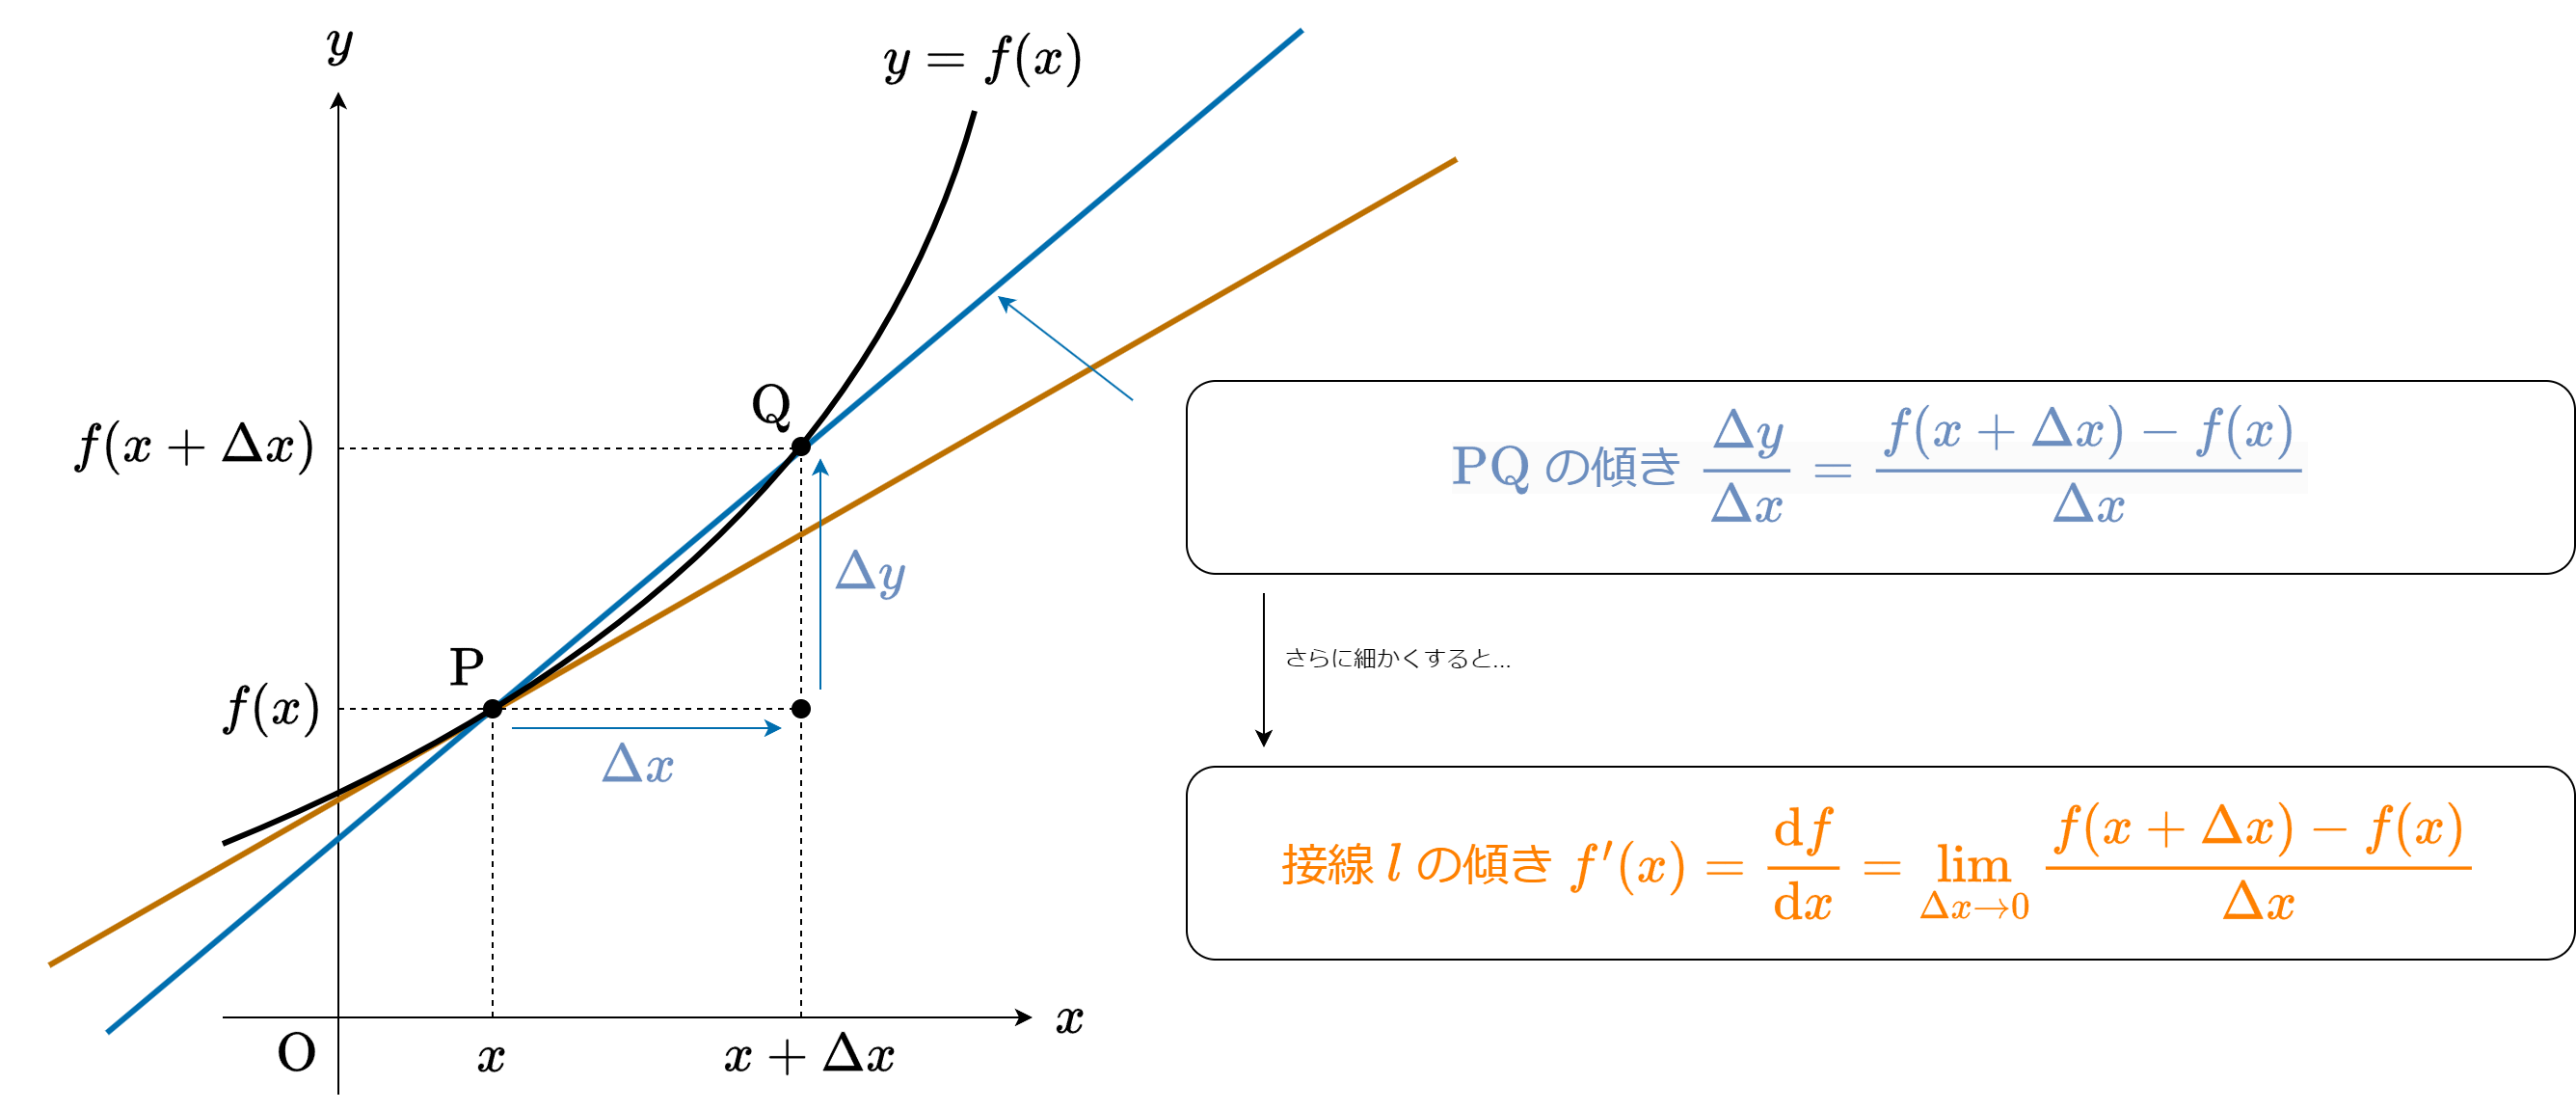
\includegraphics[width=1.0\linewidth]{img/meening-of-derivative}
		\end{figure}
	\end{frame}
	\begin{frame}{関数の微分公式(抜粋)}
		$ x $を変数、$ c $を定数とする。$ e $は\alert{ネイピア数}という定数で、$ e \simeq 2.71828\dots $
		\begin{itemize}
			\item $ \dfrac{\mathrm{d}(c)}{\mathrm{d}x} = 0 $
			\item $ \dfrac{\mathrm{d}(x)}{\mathrm{d}x} = 1 $
			\item $ \dfrac{\mathrm{d}(x^2)}{\mathrm{d}x} = 2x $
			\item $ \dfrac{\mathrm{d}(e^x)}{\mathrm{d}x} = e^x $
			\item $ \dfrac{\mathrm{d}(e^{-x})}{\mathrm{d}x} = -e^{-x} $
		\end{itemize}
	\end{frame}
	\begin{frame}{微分の性質}
		\begin{itemize}
			\item $ \{f(x)+g(x)\}' = f'(x) + g'(x) $
			\item $ \{c f(x)\}' = c f'(x) $($ c $:定数)
		\end{itemize}
		\underline{例}
		
		$ C = (2-y)^2 $($ y $:変数)のとき、
		\begin{equation*}
			\dfrac{\mathrm{d}C}{\mathrm{d}y} = \dfrac{\mathrm{d}}{\mathrm{d}y}C = \dfrac{\mathrm{d}}{\mathrm{d}y} (4 - 4y + y^2) = \dfrac{\mathrm{d}(4)}{\mathrm{d}y} - \dfrac{\mathrm{d}(4y)}{\mathrm{d}y} + \dfrac{\mathrm{d}(y^2)}{\mathrm{d}y} = 0-4+2y = -4+2y.
		\end{equation*}
	\end{frame}
	\begin{frame}{【重要】シグモイド関数$ \sigma $の微分公式}
		\begin{screen}
			$ \sigma(z) = \dfrac{1}{1 + e^{-z}} $($ z $:変数)のとき、
			\begin{equation*}
				\dfrac{\mathrm{d}\sigma(z)}{\mathrm{d}z} = \sigma(z)(1-\sigma(z))
			\end{equation*}
		\end{screen}
		\underline{ポイント}
		\begin{itemize}
			\item 導関数の値が欲しいときに、微分計算をせずに済む!
			\begin{itemize}
				\item つまり、計算機でも微分の値を容易に計算できる!
			\end{itemize}
		\end{itemize}
	\end{frame}
	\begin{frame}{【重要】関数の最小値の条件}
		\begin{screen}
			関数$ f(x) $が$ x=a $で最小値を取るとき、$ \dfrac{\mathrm{d}f(a)}{\mathrm{d}x} = 0 $
		\end{screen}
		% TODO: \usepackage{graphicx} required
		\begin{figure}
			\centering
			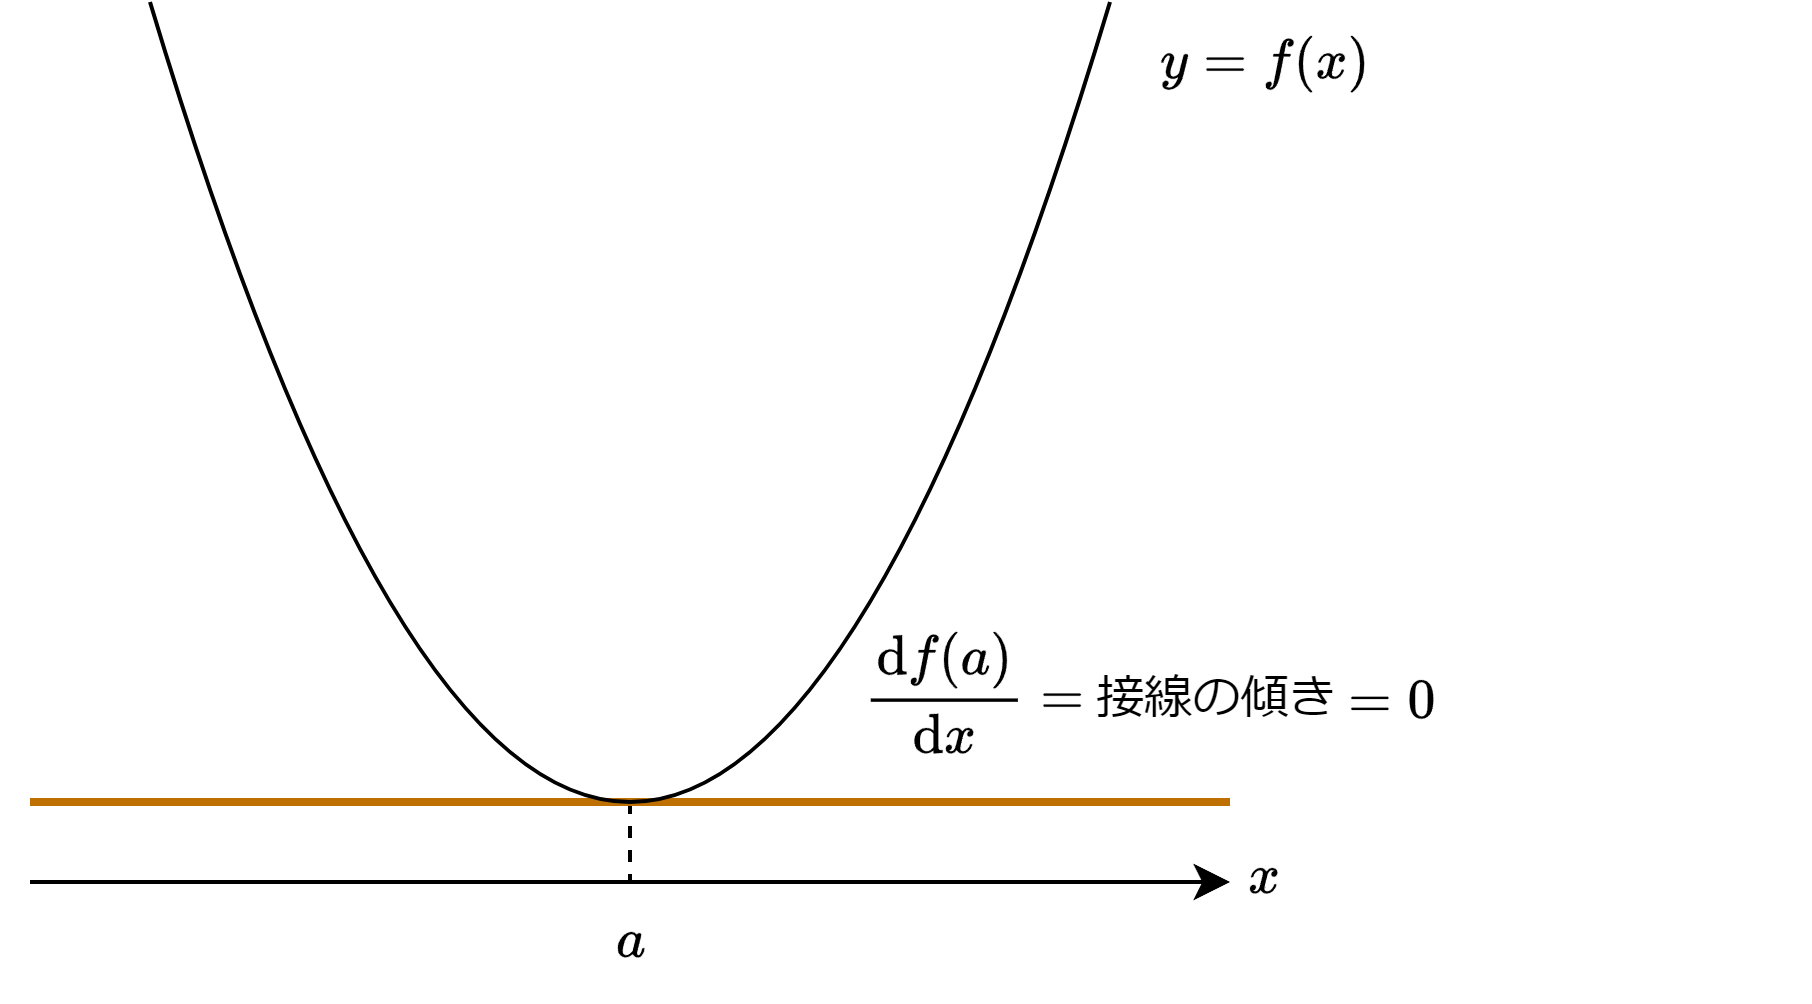
\includegraphics[width=0.7\linewidth]{img/condition-for-minimum-value-of-function}
		\end{figure}
	\end{frame}
	\begin{frame}{【重要】関数の最小値の条件}
		\begin{screen}
			$ f'(a)=0 $は関数$ f(x) $が$ x=a $で最小値になるための\underline{必要条件}である。
		\end{screen}
		% TODO: \usepackage{graphicx} required
		\begin{figure}
			\centering
			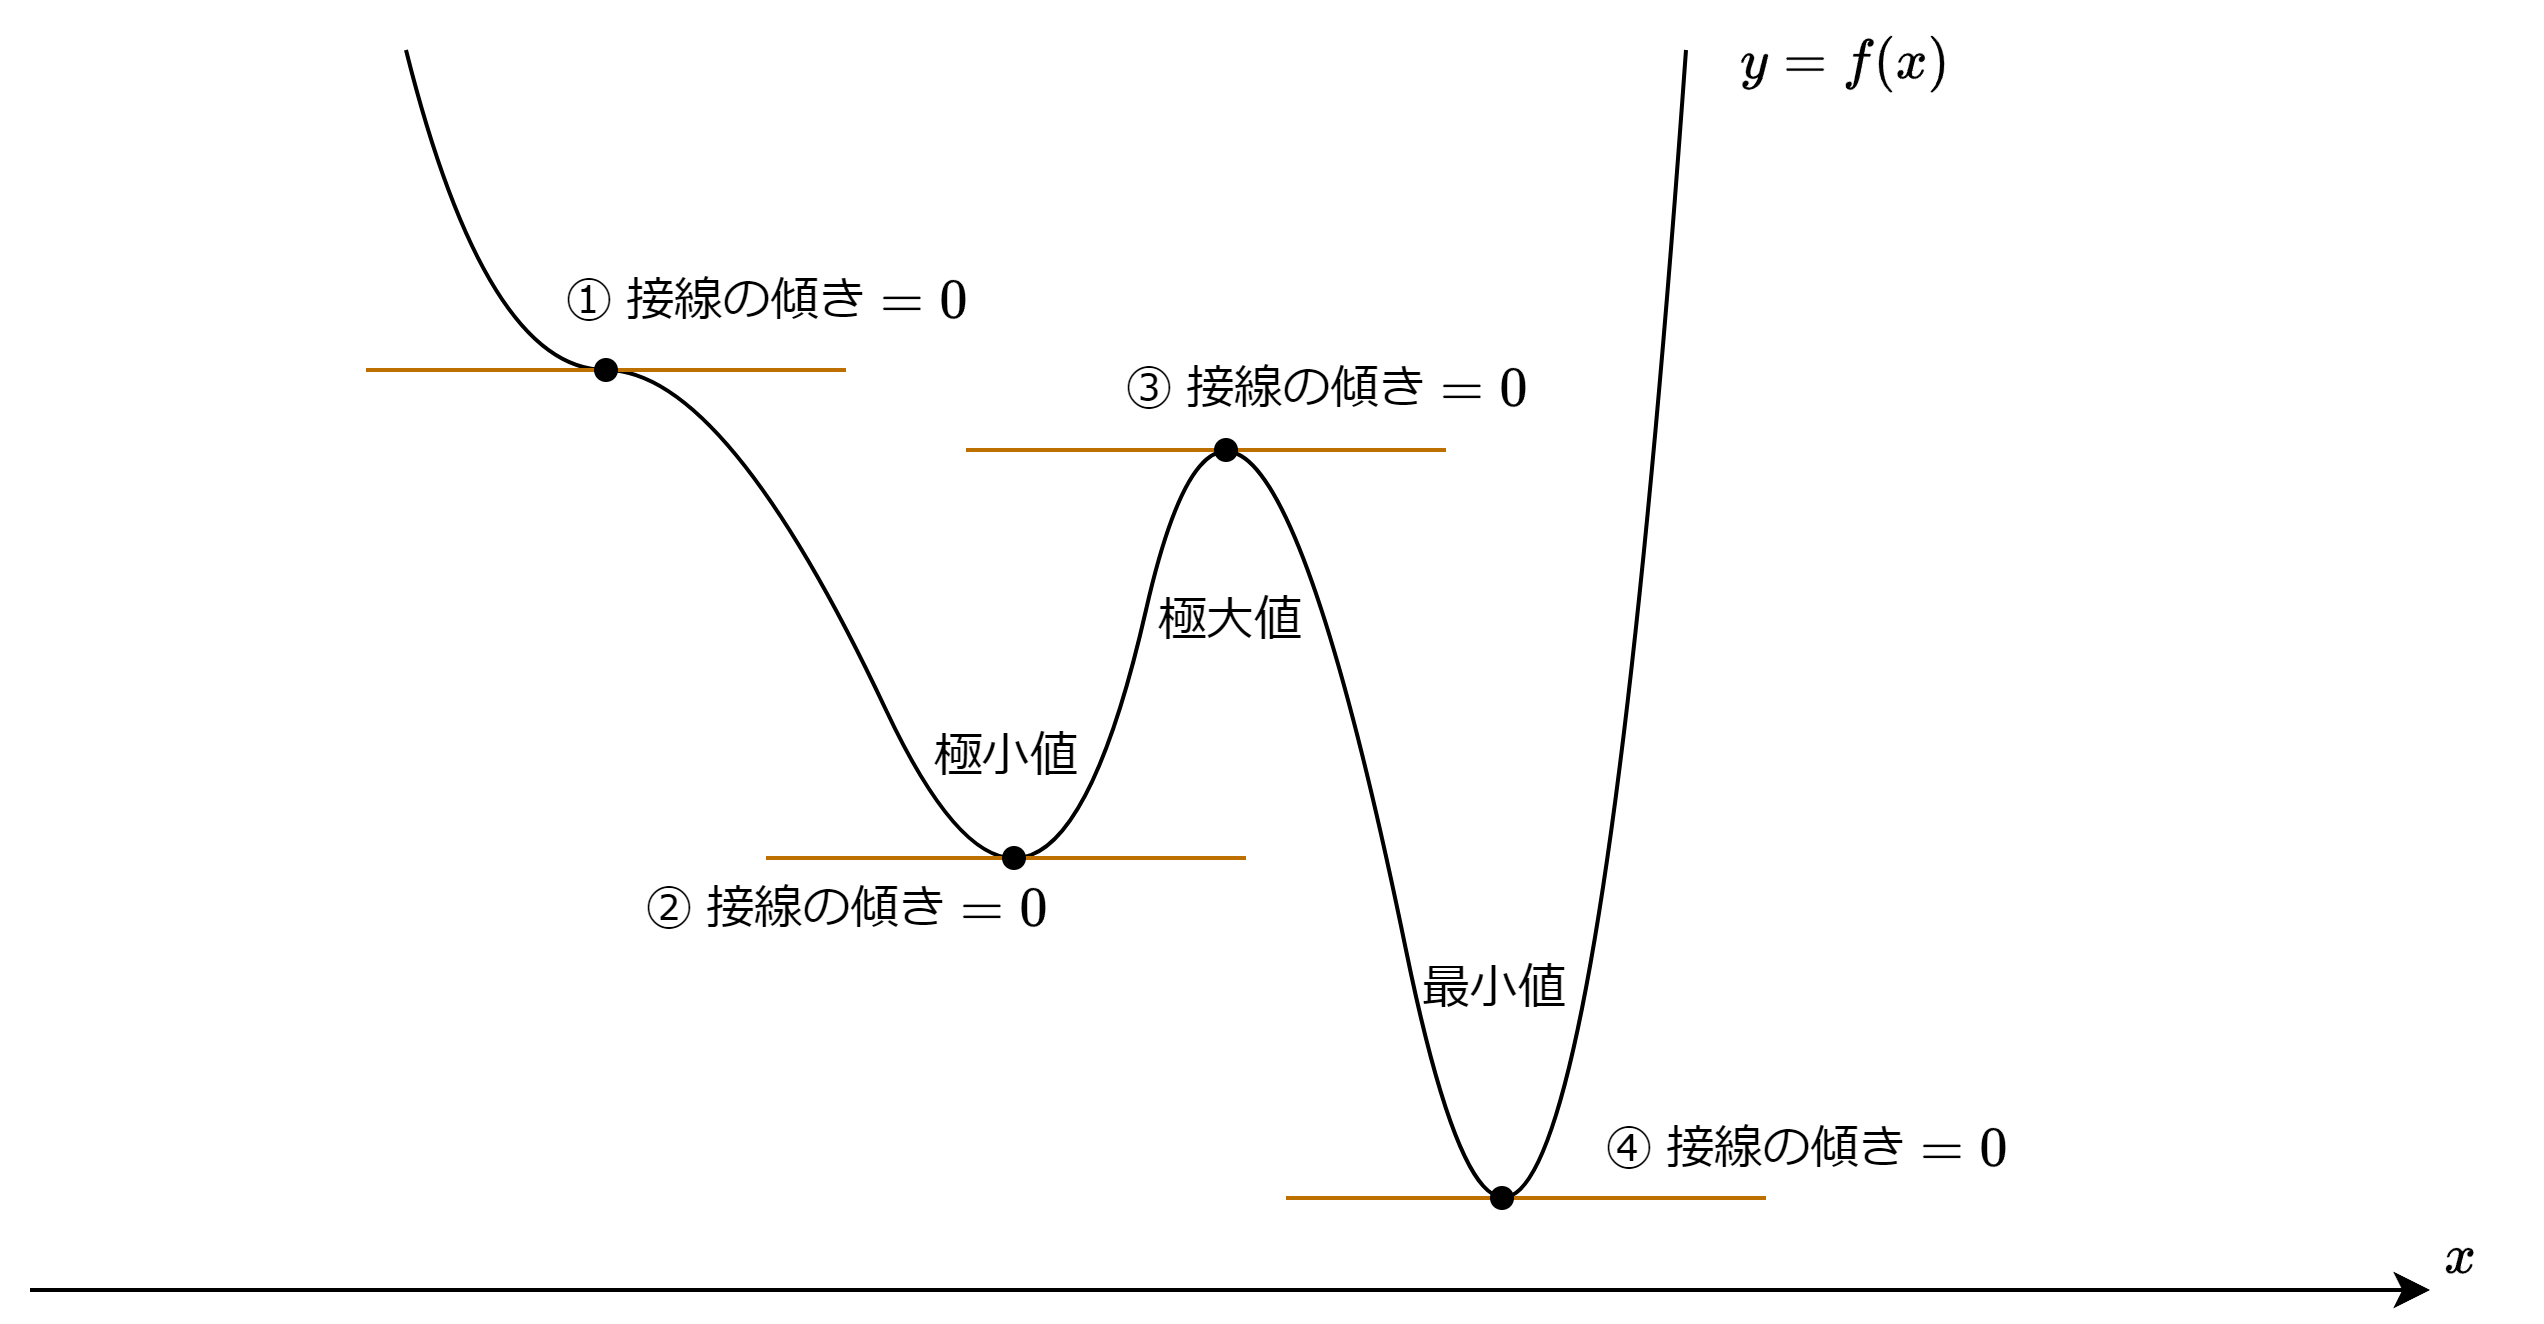
\includegraphics[width=0.7\linewidth]{img/necessary-condition-for-the-function-to-be-minimal}
		\end{figure}
	\end{frame}
	
	\subsubsection{偏微分}
	\begin{frame}{多変数関数}
		入力が2つ以上ある関数を\alert{多変数関数}という。
		\begin{figure}
			\centering
			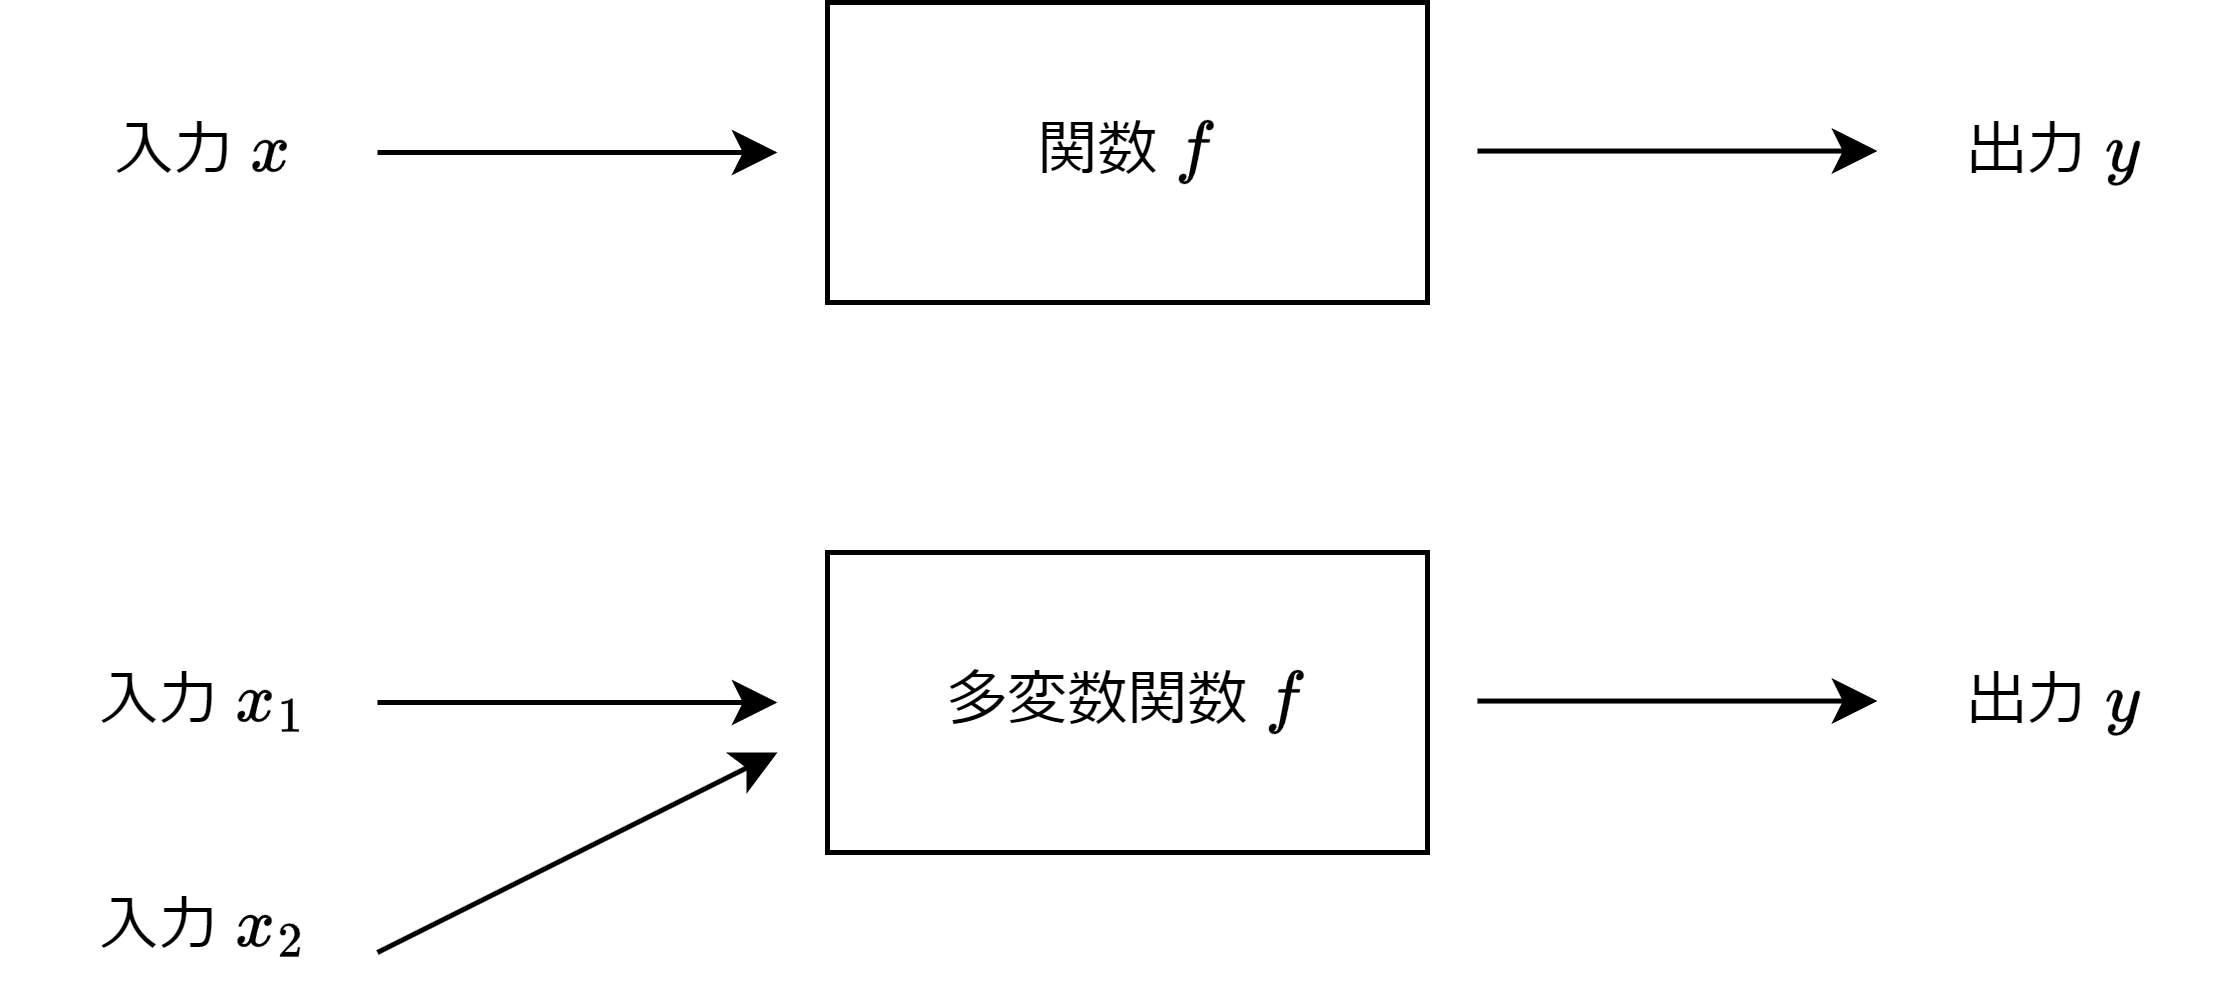
\includegraphics[width=0.7\linewidth]{img/explanation-of-mutivariate-function}
		\end{figure}
	\end{frame}
	\begin{frame}{偏微分}
		ある特定の変数について微分することを\alert{偏微分}(partial derivative)という。
		
		$ y=f(x) $を$ x $について微分する場合:
		\begin{itemize}
			\item $ \dfrac{\mathrm{d}f(x)}{\mathrm{d}x} $
		\end{itemize}
		
		$ z=f(x,y) $を$ x $について偏微分する場合:
		\begin{itemize}
			\item $ \dfrac{\partial f(x, y)}{\partial x} $
		\end{itemize}
	
		\underline{例} $ z = wx+b $のとき、$ \dfrac{\partial z}{\partial x} = w,\ \dfrac{\partial z}{\partial w} = x,\ \dfrac{\partial z}{\partial b} = 1 $
	\end{frame}
	\begin{frame}{【重要】多変数関数の最小条件}
		\begin{screen}
			関数$ z = f(x, y) $が最小になる必要条件は、$ \dfrac{\partial f}{\partial x} = 0 $かつ$ \dfrac{\partial f}{\partial y} = 0 $
		\end{screen}
		\underline{ポイント}
		
		どの成分から見ても傾きが$ 0 $なら、最小値の可能性あり!
	\end{frame}
	
	\subsubsection{関数の近似公式}
	\begin{frame}{関数の近似公式}
		1変数関数の場合
		\begin{screen}
			$ f(x+\Delta x) \simeq f(x) + f'(x)\Delta x $
		\end{screen}
		2変数関数の場合
		\begin{screen}
			$ f(x+\Delta x,\ y+\Delta y) \simeq f(x,y) + \dfrac{\partial f(x,y)}{\partial x}\Delta x + \dfrac{\partial f(x,y)}{\partial y}\Delta y $
		\end{screen}
		※$ \Delta x $や$ \Delta y $は十分小さな数とする。
	\end{frame}
	\begin{frame}[shrink]{【重要】関数の近似公式 簡潔 ver.}
		\begin{screen}
			$ \Delta z \triangleq f(x_1+\Delta x_1,\ x_2+\Delta x_2) - f(x_1,\ x_2) $とすると、
			\begin{equation*}
				\Delta z \simeq \dfrac{\partial z}{\partial x_1} \Delta x_1 + \dfrac{\partial z}{\partial x_2} \Delta x_2.
			\end{equation*}
			$ \nabla z \triangleq \begin{bmatrix}
				\dfrac{\partial z}{\partial x_1}\vspace{0.5em}\\
				\dfrac{\partial z}{\partial x_2}
			\end{bmatrix},\ \Delta \boldsymbol{x} \triangleq \begin{bmatrix}
				\Delta x_1\\
				\Delta x_2
			\end{bmatrix} $とすると、
			\begin{equation*}
				\Delta z \simeq \left\langle \nabla z,\ \Delta \boldsymbol{x} \right\rangle.
			\end{equation*}
		\end{screen}
		
		\underline{ポイント} 
		
		関数の値の変化$ \Delta z $は、偏微分を集めたベクトル$ \nabla z $と、小さい値を集めたベクトル$ \Delta \boldsymbol{x} $で表される。
	\end{frame}
	
	\subsection{誤差逆伝播法のための数学}
	\subsubsection{連鎖律}
	\begin{frame}{合成関数}
		入れ子構造の関数$ f(g(x)) $を、関数$ f $と$ g $の\alert{合成関数}という。
		% TODO: \usepackage{graphicx} required
		\begin{figure}
			\centering
			
\includegraphics[width=0.7\linewidth]{img/composite-function}
		\end{figure}
	\end{frame}
	\begin{frame}{1変数関数の連鎖律}
		\begin{screen}
			1変数関数$ y = f(u) $があり、その$ u $が1変数関数$ u = g(x) $と表されるとき、合成関数$ f(g(x)) $の導関数は次のように求められる:
			\begin{equation*}
				\dfrac{\mathrm{d}y}{\mathrm{d}x} = \dfrac{\mathrm{d}y}{\mathrm{d}u} \cdot \dfrac{\mathrm{d}u}{\mathrm{d}x}
			\end{equation*}
		\end{screen}
					% TODO: \usepackage{graphicx} required
		\begin{figure}
			\centering
			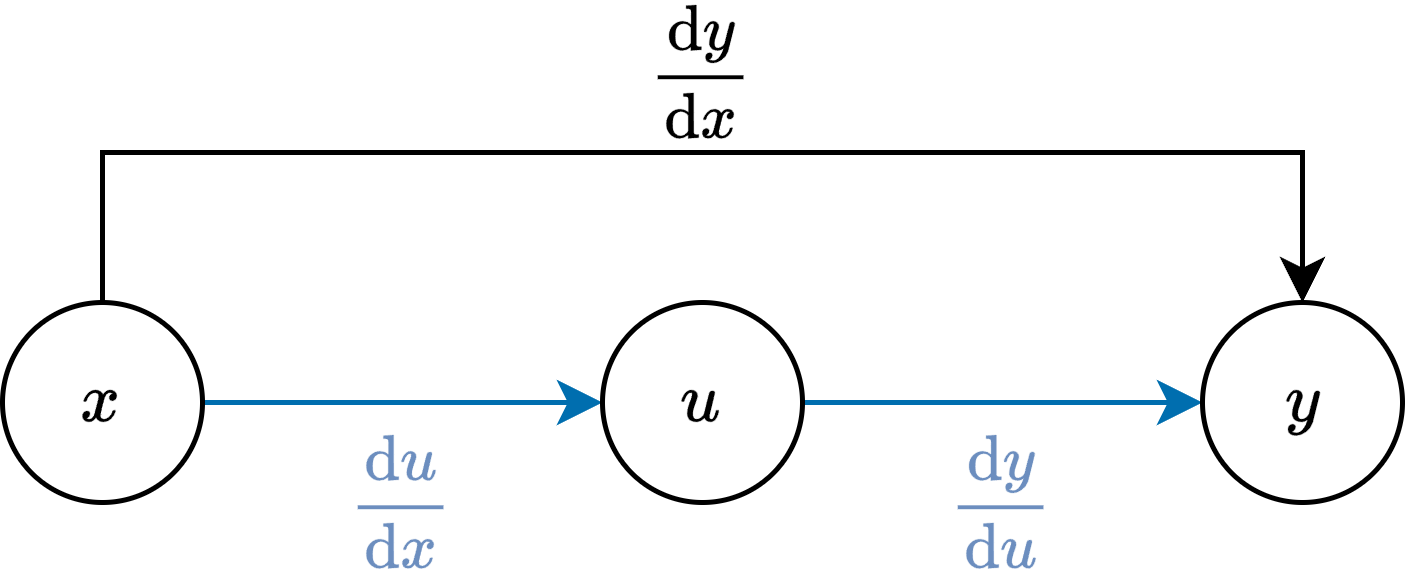
\includegraphics[width=0.65\linewidth]{img/chain-rule-at-1-variable}
		\end{figure}
	\end{frame}
	\begin{frame}{1変数関数の連鎖律の例}
		$ y = u^2,\ u = 2-x $のとき、$ y $を$ x $で微分すると、
		\begin{align*}
			\dfrac{\mathrm{d}y}{\mathrm{d}x} = \dfrac{\mathrm{d}y}{\mathrm{d}u} \dfrac{\mathrm{d}u}{\mathrm{d}x} = \dfrac{\mathrm{d}(u^2)}{\mathrm{d}u} \dfrac{\mathrm{d}(2-x)}{\mathrm{d}x} = 2u \cdot (-1) = -2u = -2(2-x) = -4+2x.
		\end{align*}
	\end{frame}
	\begin{frame}{2変数関数の連鎖律}
		\begin{screen}
			2変数関数$ z = f(u,v) $があり、その$ u,\ v $が2変数関数$ u = g_1(x,y),\ v = g_2(x,y) $と表されるとき、
			\begin{equation*}
				\dfrac{\partial z}{\partial x} = \dfrac{\partial z}{\partial u}\cdot\dfrac{\partial u}{\partial x} + \dfrac{\partial z}{\partial v}\cdot\dfrac{\partial v}{\partial x}
			\end{equation*}
		\end{screen}
		% TODO: \usepackage{graphicx} required
		\begin{figure}
			\centering
			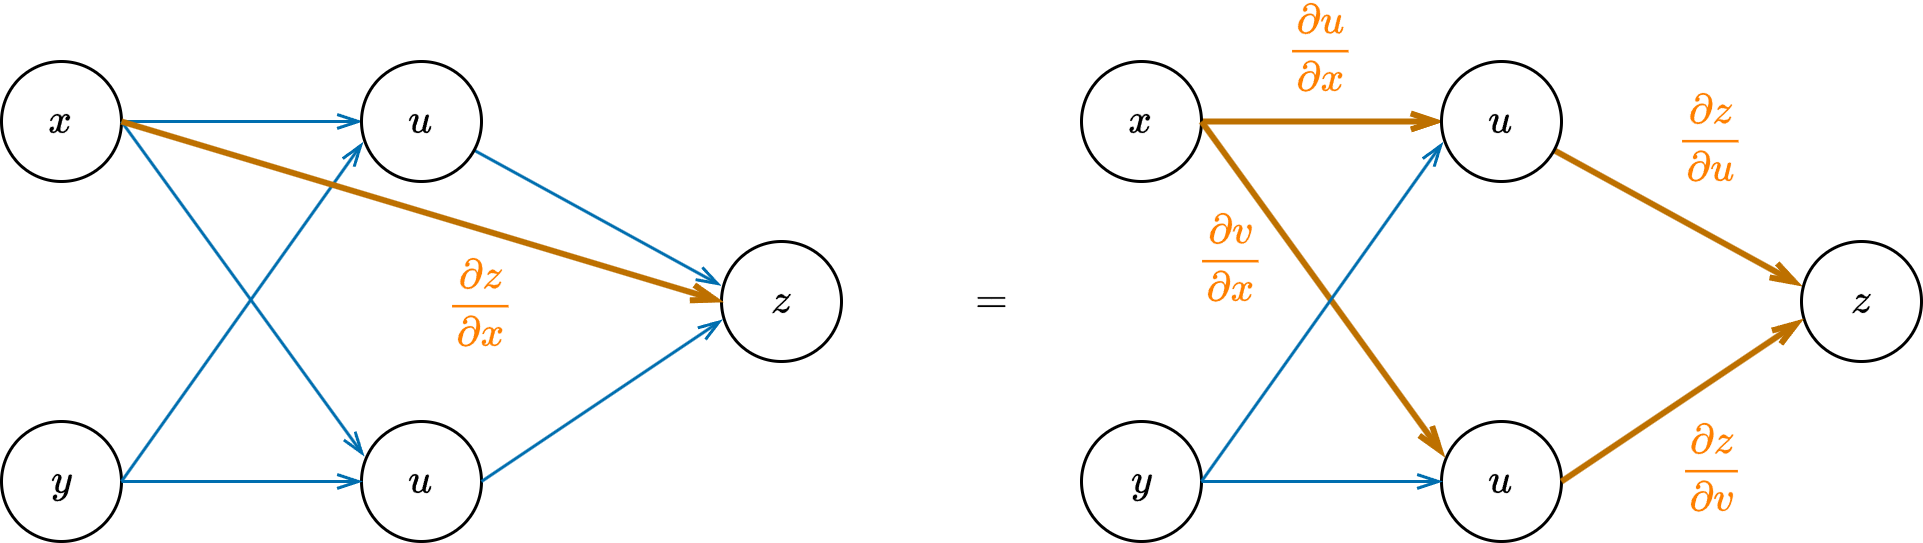
\includegraphics[width=0.8\linewidth]{img/chain-rule-of-multivariable-functions}
		\end{figure}
	\end{frame}
	\begin{frame}{2変数関数の連鎖律の例}
		$ z=u^2+v^2,\ u=ax+by,\ v=px+qy $($ a, b, p, q $:定数)のとき、
		\begin{align*}
			\dfrac{\partial z}{\partial x} = \dfrac{\partial z}{\partial u}\dfrac{\partial u}{\partial x} + \dfrac{\partial z}{\partial v}\dfrac{\partial v}{\partial x} = 2u \cdot a + 2v \cdot p = 2a(ax+by) + 2p(px+qy).
		\end{align*}
	\end{frame}
	
\end{document}
